\documentclass{article}
\usepackage{graphicx, xcolor}
\usepackage{subcaption}
\usepackage{amsmath}
\usepackage{hyperref}
\hypersetup{hidelinks}
\usepackage{listings}
\usepackage{caption}
\usepackage{float}
\usepackage{booktabs}
\usepackage[margin=2.5cm]{geometry}

\title{Praktické paralelní programování\\Dokumentace k projektu č. 1\\MPI a paralelní I/O}
\author{Dominik Huml (xhumld00)}
\date{\today}

\begin{document}

\maketitle

% =========================================================
\section{Úvod}
\label{sec:uvod}
% =========================================================

Projekt implementuje paralelní simulaci šíření tepla 2D doménou pomocí
metody konečných diferencí (FDTD).
Paralelizace je realizována kombinací MPI (rozdělení domény mezi procesy)
a OpenMP (vlákna uvnitř procesu). Výměna halo zón je implementována dvěma způsoby (P2P a RMA).
Průběh simulace je ukládán do souboru HDF5 s podporou paralelního zápisu.

% =========================================================
\section{Popis implementace}
\label{sec:implementace}
% =========================================================

\subsection*{Dekompozice domény}
Implementace podporuje 1D dekompozici ($n_x = P$, $n_y = 1$, dělení pouze v jednom směru)
a 2D dekompozici (čtvercové nebo obdélníkové dlaždice dle parity $\log_2 P$).
Topologie procesů je kartézská (\texttt{MPI\_Cart\_create}).
Komunikační skupina je určena pomocí \texttt{MPI\_Cart\_shift}.

\subsection*{Překrytí výpočtu a komunikace}
Každá iterace probíhá ve čtyřech fázích,
(1)~\texttt{computeHaloZones} vypočítá okrajové buňky dlaždice (data k odeslání),
(2)~\texttt{startHaloExchange\{RMA | P2P\}} zahájí neblokující výměnu halo zón,
(3)~\texttt{updateTile} aktualizuje vnitřek dlaždice za běhu přenosu,
(4)~\texttt{awaitHaloExchange\{RMA | P2P\}} čeká na dokončení výměny.
Část komunikace tak může probíhat souběžně s výpočtem vnitřní části dlaždice.
Přínos překrytí roste s poměrem vnitřku dlaždice k halo zóně:
pro 2D dlaždici strany $L = N/\sqrt{P}$ je tento poměr přibližně $L/8$.
Při $L = 1024$ (16 procesů, doména $4096^2$) je vnitřek dlaždice
\textbf{128$\times$} větší než halo, takže překrytí má dostatečný výpočetní prostor.

\subsection*{RMA implementace s MPI\_Put, packingem a PSCW}
Pro RMA halo výměnu byly experimentálně porovnány dva přístupy.
Varianta s \texttt{MPI\_Get} a strided MPI datovými typy (přímé čtení
z paměti souseda) se na architektuře Cascade Lake s Intel MPI RDMA
cestou ukázala jako extrémně pomalá, naměřeno 55-80$\times$ zpomalení
oproti variantě s \texttt{MPI\_Put}.
Zvolená implementace proto používá \texttt{MPI\_Put}, kdy každý proces
\emph{zapisuje} svá halo data do okna souseda.
Data jsou před přenosem zabalena pomocí \texttt{MPI\_Pack/Unpack}
do spojitého bufferu, čímž se eliminují strided přístupy.
Pro synchronizaci je použit protokol PSCW
(\texttt{MPI\_Win\_post/start/complete/wait}), který synchronizuje pouze
přímé sousedy dlaždice namísto globální bariéry \texttt{MPI\_Win\_fence}.

Příspěvky jednotlivých optimalizací k celkovému zrychlení RMA
(16 procesů, 1-2 uzly, variabilní velikosti dlaždic):

\begin{center}
\begin{tabular}{lr}
\toprule
Optimalizace & Zrychlení \\
\midrule
\texttt{MPI\_Get} $\to$ \texttt{MPI\_Put} & 55-80$\times$ \\
Packing (\texttt{MPI\_Pack/Unpack})        & 1{,}5-3$\times$ \\
Fence $\to$ PSCW (1 uzel)                 & 1{,}15$\times$ \\
Fence $\to$ PSCW (2 uzly)                 & 1{,}74$\times$ \\
\midrule
\multicolumn{2}{l}{\textit{Kombinovaný efekt (naive $\to$ optimalizováno)}} \\
\quad 2D, 1 uzel & 164$\times$ \\
\quad 1D, 1 uzel & 268$\times$ \\
\quad 2D, 2 uzly & 133$\times$ \\
\bottomrule
\end{tabular}
\end{center}

\subsection*{Paralelní I/O a HDF5 chunkování}
Parametr \texttt{H5Pset\_chunk} určuje, jak HDF5 rozdělí dataset do bloků.
Nastavení tohoto parametru na rozměr celé globální domény zajistí
jeden společný blok pro všechny procesy a umožní skutečně kolektivní zápis.
Při nastavení odpovídajícím lokální dlaždici vzniká velké množství malých
nezávislých bloků, což při vyšším počtu MPI procesů vede k mnohonásobně
delším časům zápisu. Nastavení \texttt{H5Pset\_chunk} na rozměr celé domény
v kombinaci s Lustre stripingem (\texttt{lfs setstripe -S 1M -c 16})
přineslo \textbf{řádové zrychlení oproti původní paralelní variantě
s lokálními chunky}.

% =========================================================
\section{Škálování}
\label{sec:skalovani}
% =========================================================

Silné škálování je měřeno na mřížkách 256-4096 při 1-128 procesech
(MPI 2D) resp. 1-32 MPI procesů $\times$ 8 vláken (Hybrid 2D) nebo
1-16 MPI procesů $\times$ 16 vláken (Hybrid 1D), celkem až 256 jader
na 8 uzlech Barbory.
Jako referenční čas slouží sekvenční implementace na téže velikosti domény.
Pro doménu $4096^2$ je sekvenční čas 53{,}6\,s / 488 iterací
$\approx 0{,}110$\,s/iteraci.

Nejlepší naměřené zrychlení:
\begin{center}
\begin{tabular}{lrrr}
\toprule
Konfigurace & Jader & Čas/iteraci [s] & Zrychlení \\
\midrule
Hybrid 2D P2P (32 MPI $\times$ 8 OMP) & 256 & $1{,}65 \times 10^{-4}$ & $\mathbf{\sim 666\times}$ \\
Hybrid 1D P2P (16 MPI $\times$ 16 OMP) & 256 & $2{,}70 \times 10^{-4}$ & $\sim 407\times$ \\
MPI 2D P2P (128 MPI $\times$ 1 OMP)   & 128 & $3{,}11 \times 10^{-4}$ & $\sim 354\times$ \\
\bottomrule
\end{tabular}
\end{center}

Zrychlení Hybrid 2D je \textbf{superlineární} vůči ideálnímu 256$\times$.
Příčinou je cache efekt. Sekvenční solver pracuje s doménou $4096^2$
($\approx 130$\,MB), která se nevejde do L3 cache (24{,}75\,MB/socket).
U 32 procesů má každá dlaždice rozměr $1024 \times 512$ floatů ($\approx 2$\,MB)
a dvě teplotní pole mají dohromady přibližně 4\,MB, takže se vejdou do L3.
Výpočet běží z cache místo RAM.

\subsection*{Rozdíl 1D a 2D dekompozice}
Klíčovým faktorem je objem komunikace na proces.
Pro $P$ procesů a mřížku $N \times N$ platí:
\[
  V_\text{1D} = 4N \quad (\text{dvě plné hrany šířky 2}),\qquad
  V_\text{2D} = \frac{8N}{\sqrt{P}} \quad (\text{čtyři kratší hrany}),\qquad
  \frac{V_\text{1D}}{V_\text{2D}} = \frac{\sqrt{P}}{2}.
\]
Při $P = 16$ posílá 1D \textbf{2$\times$} více dat, při $P = 256$
již \textbf{8$\times$} více.
V praxi Hybrid 1D dosahuje na 256 jádrech zrychlení $\approx 407\times$
oproti $\approx 666\times$ u Hybrid 2D, tj. $\sim 1{,}6\times$ horší výsledek.
Z 90 přímých srovnání (Hybrid 1D vs.\ Hybrid 2D při shodném počtu jader,
velikosti domény, komunikačním módu a režimu I/O) zvítězila 2D dekompozice
v 63 případech ($\sim$70\,\%).

\subsection*{Vyrovnanost zátěže}
Doména je rozdělena na dlaždice stejné velikosti, takže každý proces
aktualizuje shodný počet bodů. Stencil výpočet (\texttt{computePoint})
provede pevný počet operací na bod nezávisle na materiálových parametrech.
Profilování (viz sekci~\ref{sec:profilovani}) potvrzuje uniformní
rozložení jak výpočetní zátěže, tak objemu zaslaných halo dat.

\subsection*{Vliv paralelního I/O}
Naměřené časy pro Hybrid 2D P2P, 16 MPI $\times$ 8 OMP (128 jader):
\begin{center}
\begin{tabular}{lrr}
\toprule
Režim I/O & Doména $1024^2$ & Doména $4096^2$ \\
\midrule
Bez I/O    & 0{,}72\,s & 1{,}55\,s \\
Sekvenční  & 2{,}07\,s & 7{,}58\,s \\
Paralelní  & 13{,}7\,s & 25{,}9\,s \\
\bottomrule
\end{tabular}
\end{center}

Paralelní HDF5 I/O je při použitých velikostech domén pomalejší
než sekvenční zápis. Důvodem je kombinace
malých jednotlivých zápisů (4--64\,MB na snapshot) a režie Lustre OST koordinace.

\subsection*{Slabé škálování}
Velikost úlohy roste úměrně s počtem MPI procesů
(65\,536 buněk/rank, body $4 \times 512^2$ až $256 \times 4096^2$).
Iterační čas s rostoucím $P$ mírně roste u všech implementací,
což odpovídá očekávané sub-ideální efektivitě:
MPI 2D drží 82{,}2\,\% na 256 jádrech (nejstabilnější),
Hybrid 2D 78{,}5\,\% na 128 jádrech,
Hybrid 1D klesá na 55{,}5\,\% na 256 jádrech kvůli většímu komunikačnímu objemu.
Hybridní varianty mají nižší absolutní iterační čas díky OpenMP threadům
ve sdílené paměti (kratší halo zóny mezi procesy).

% ----- MPI 2D -----
\begin{figure}[H]
    \centering
    \begin{subfigure}{0.45\textwidth}
        \centering
        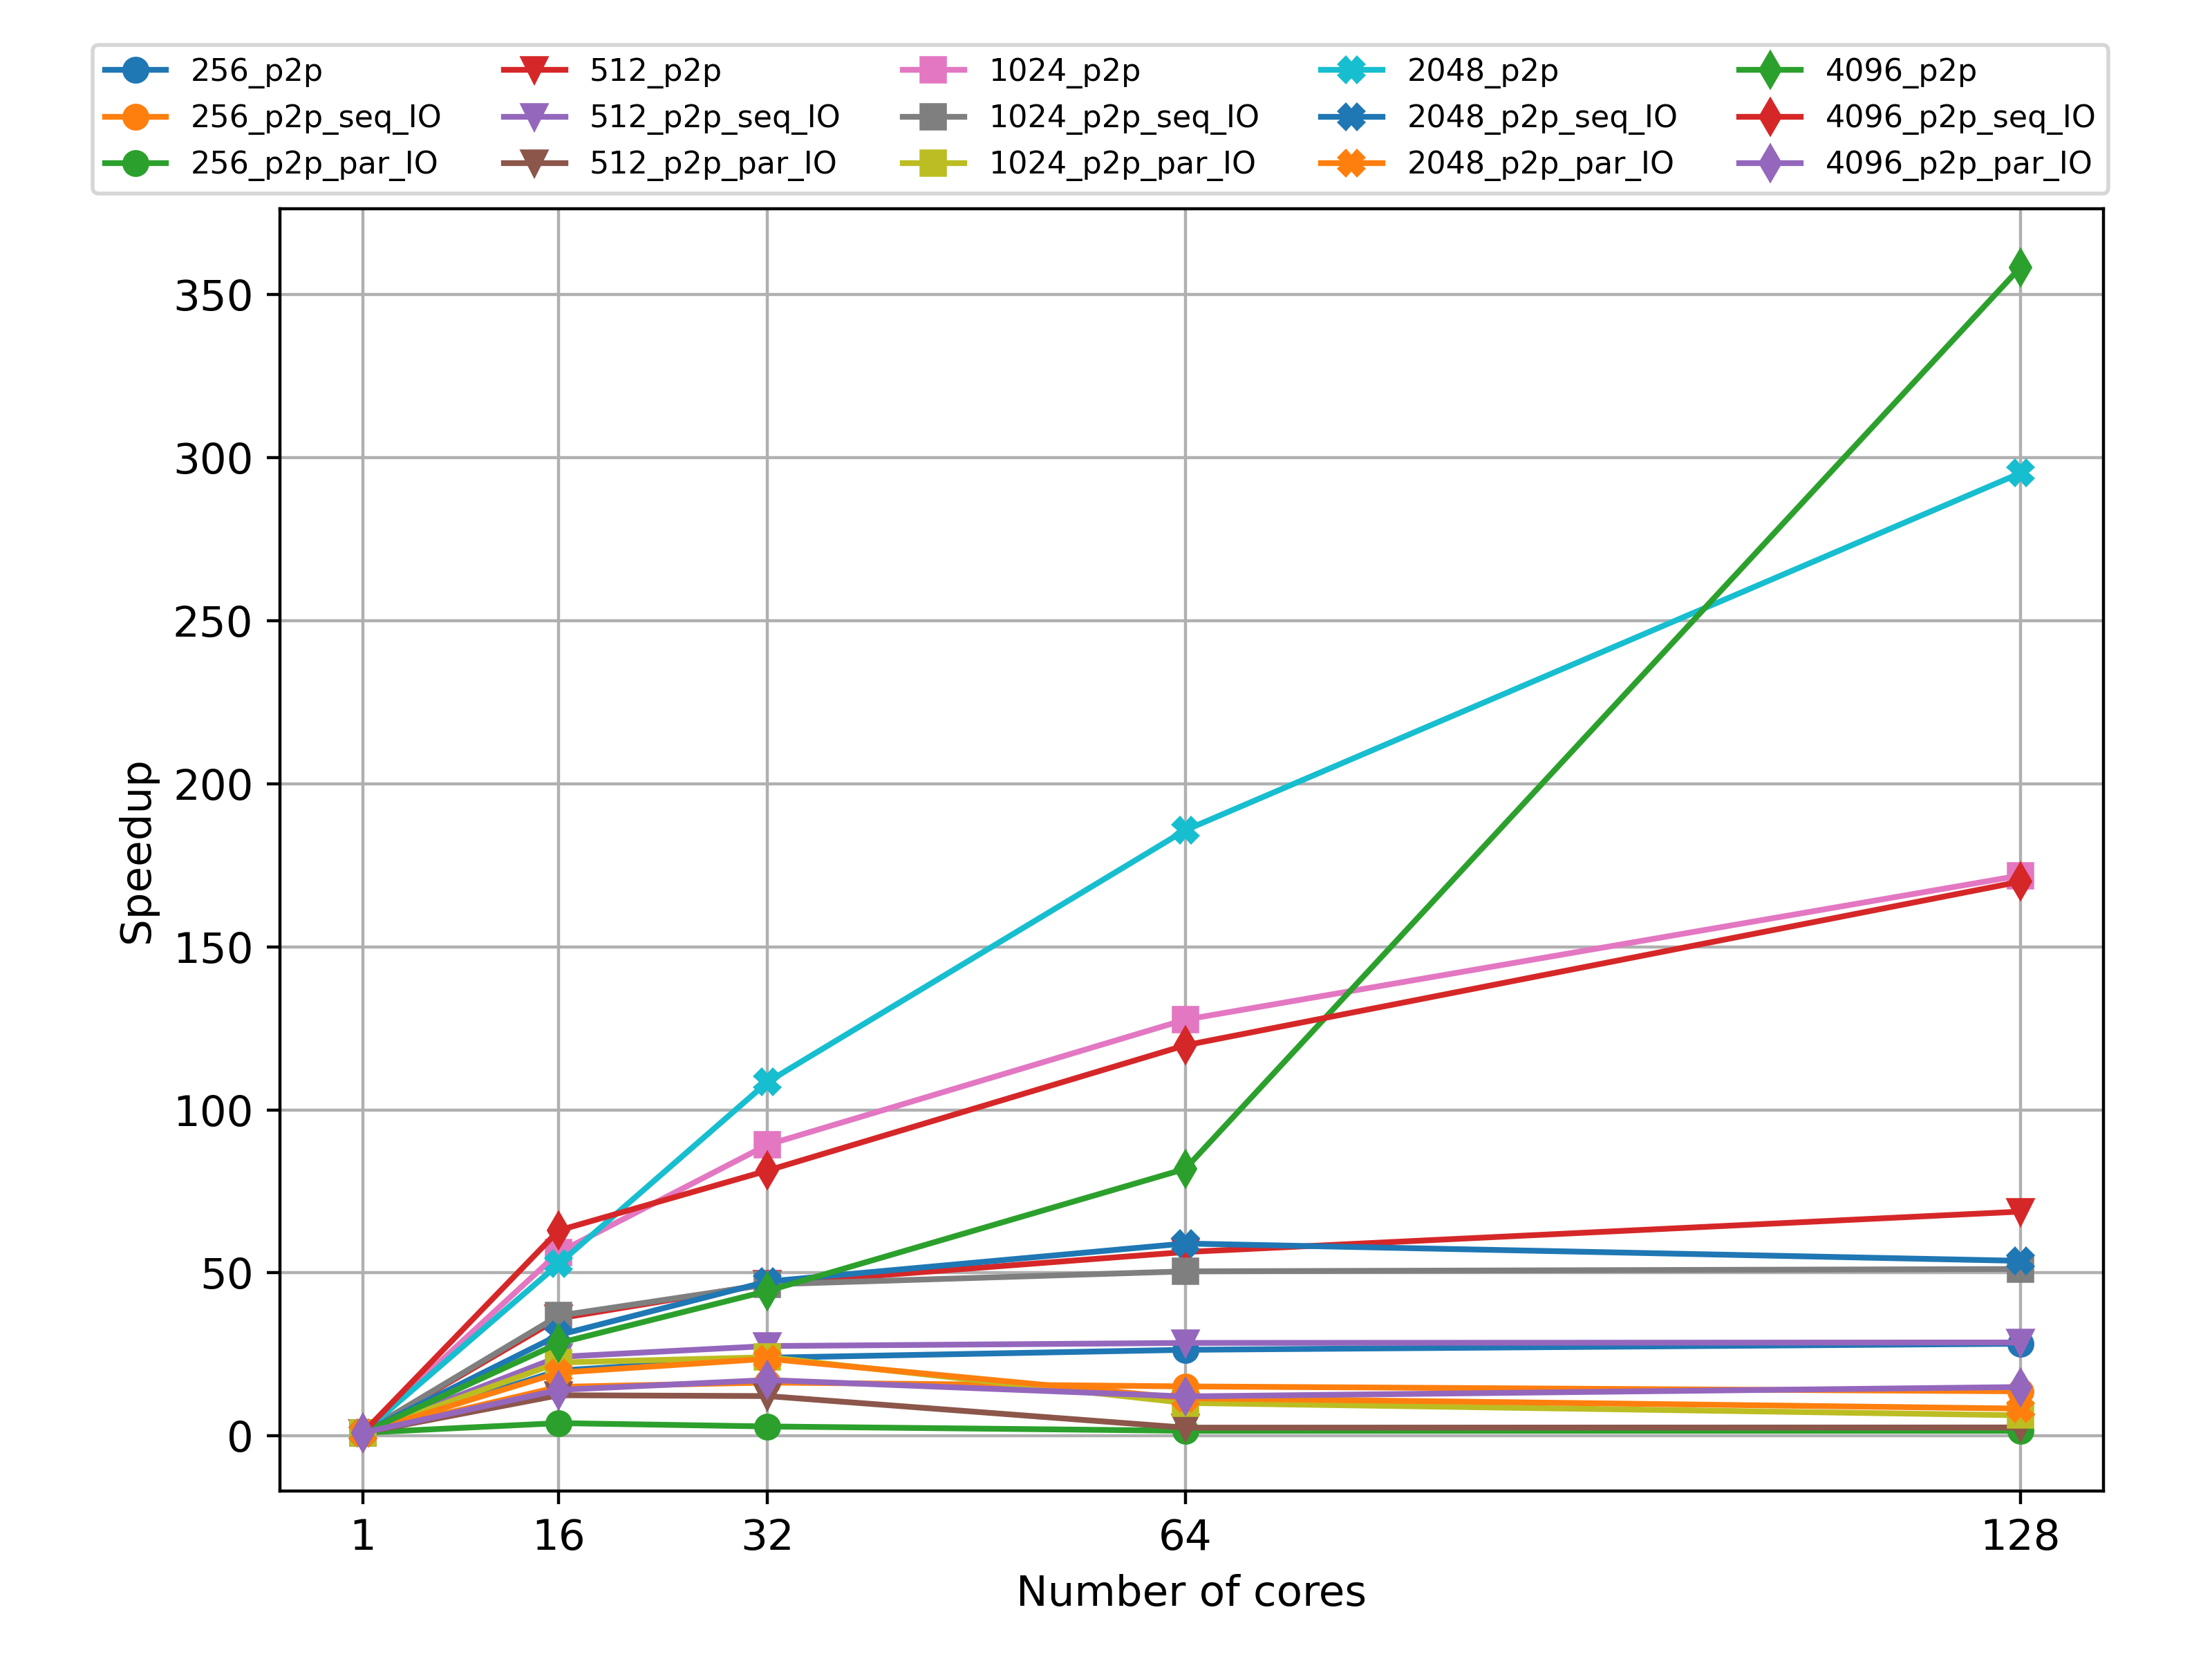
\includegraphics[width=\textwidth]{docs/figures/ppp_speedup_mpi_p2p.png}
        \caption{Silné škálování: čisté MPI s 2D dekompozicí, výměna okrajů pomocí P2P.}
        \label{fig:2D_MPI_P2P}
    \end{subfigure}
    \hfill
    \begin{subfigure}{0.45\textwidth}
        \centering
        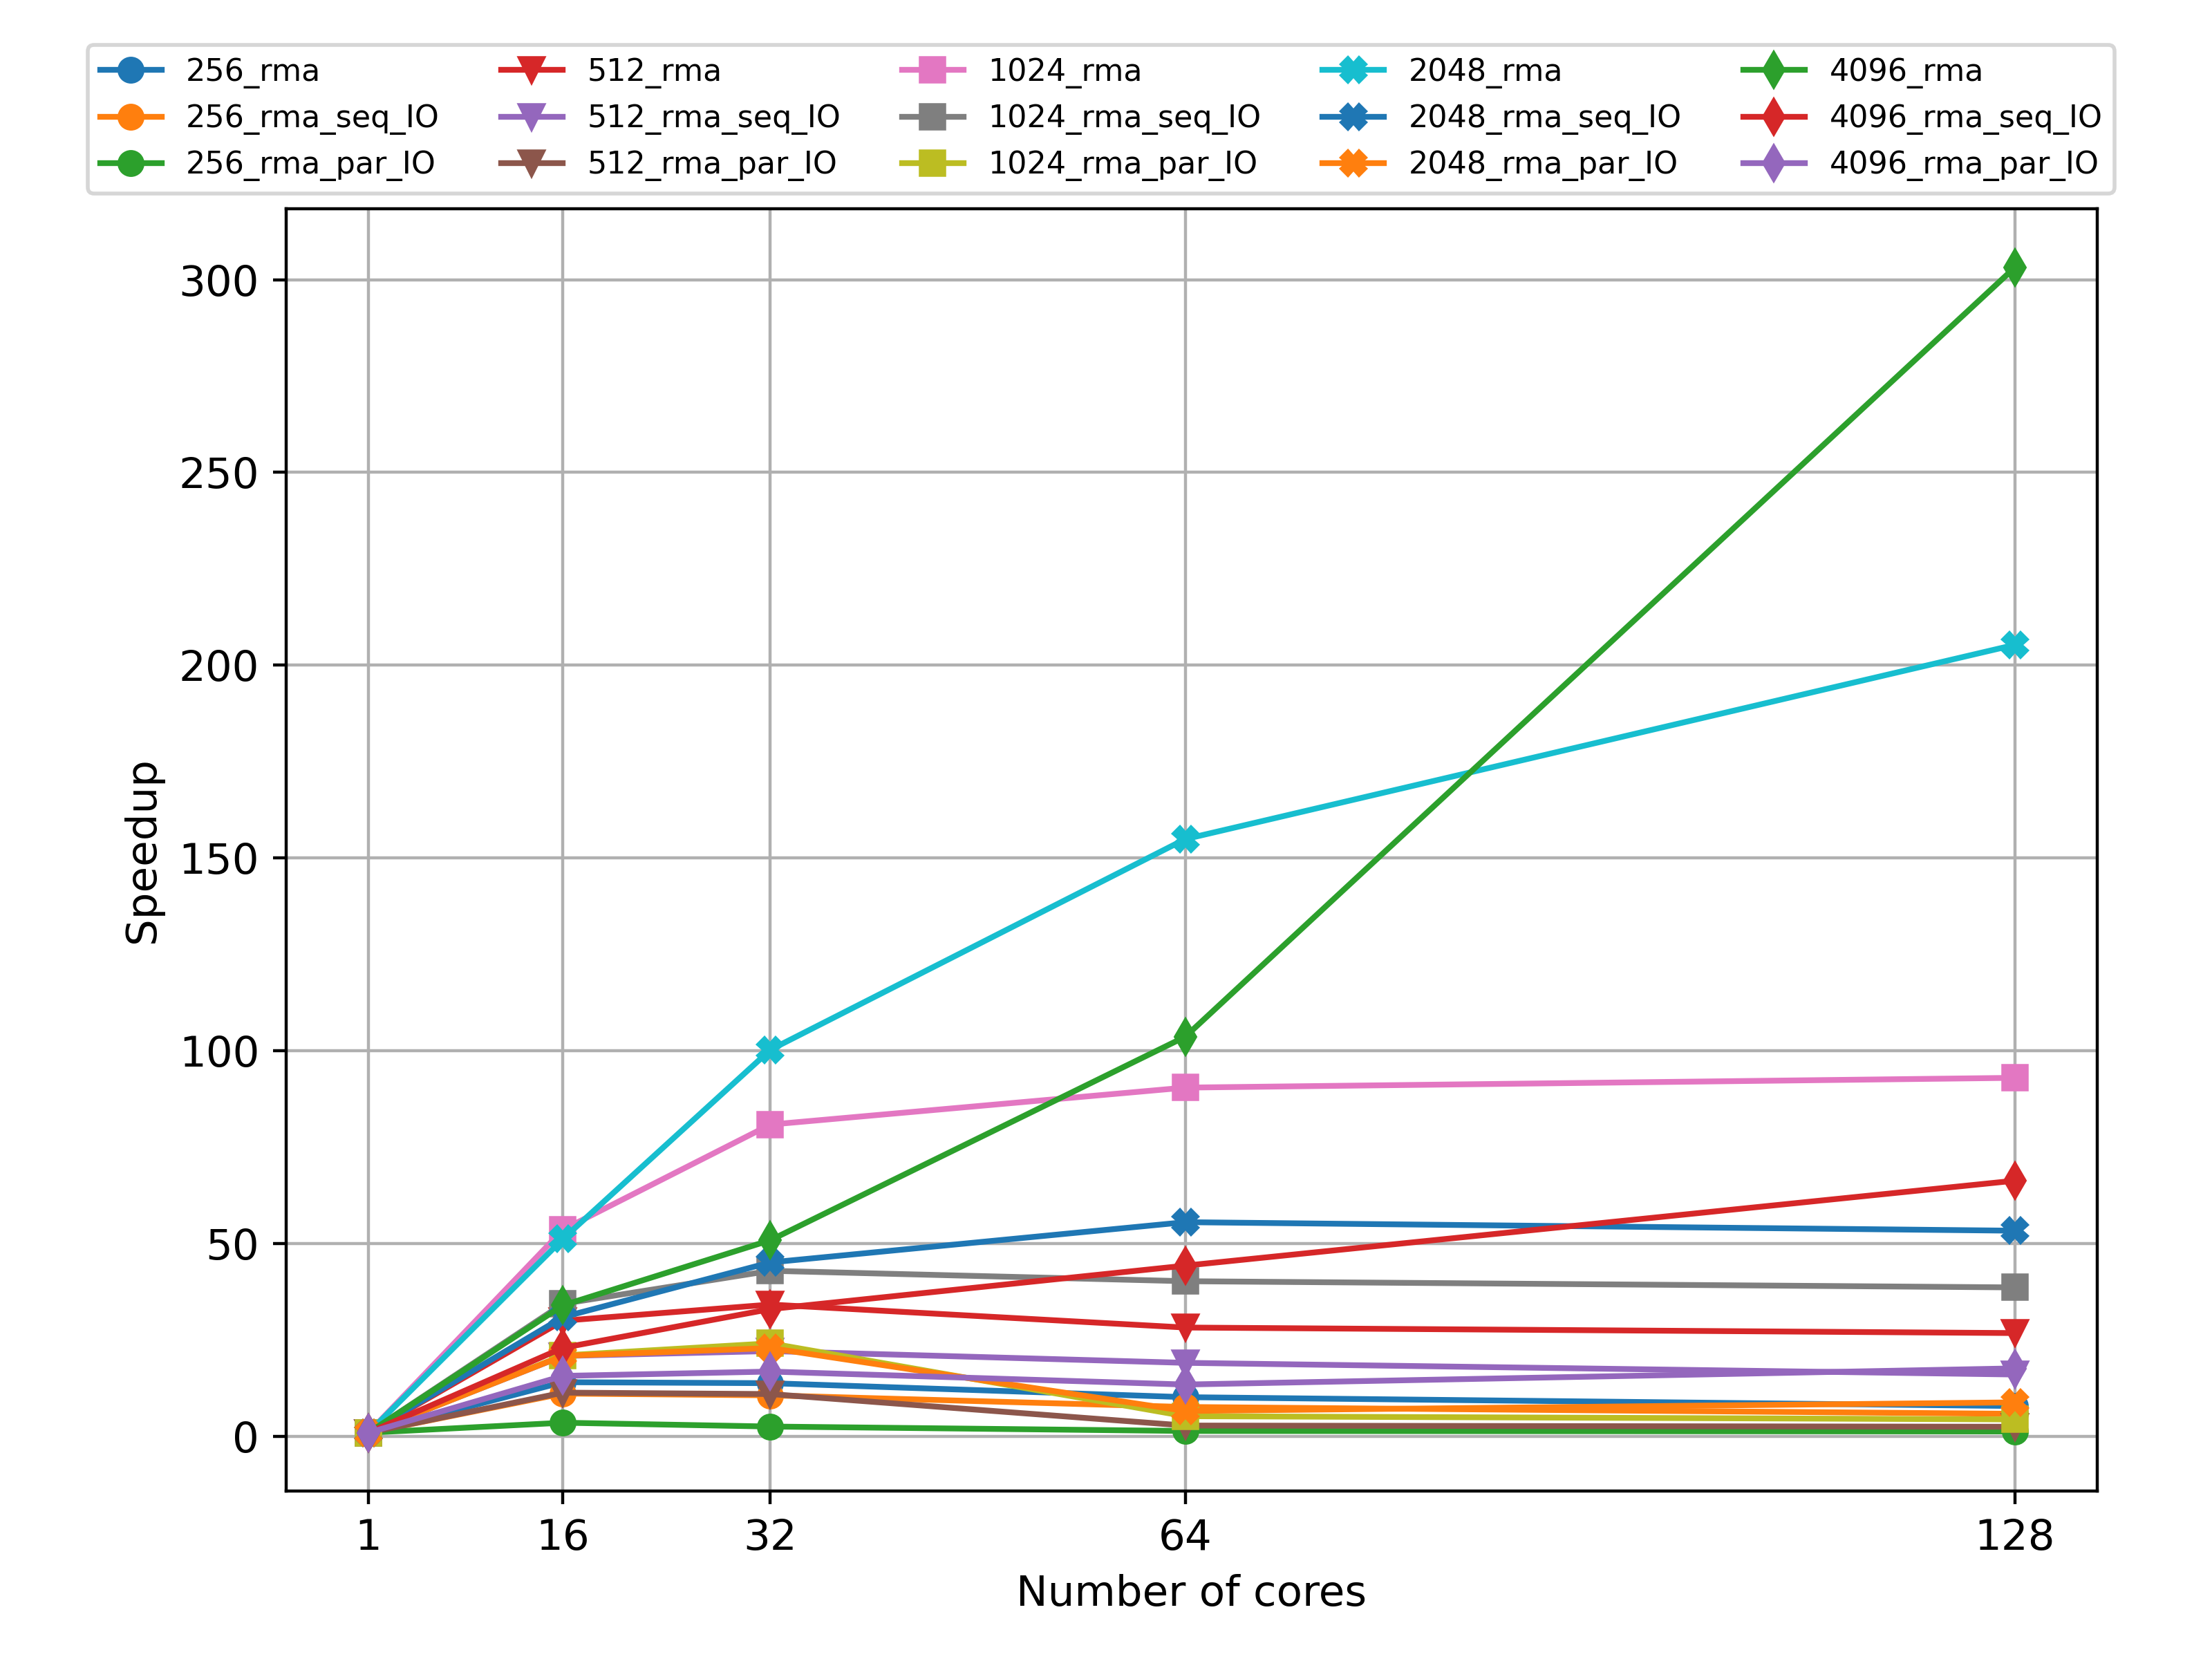
\includegraphics[width=\textwidth]{docs/figures/ppp_speedup_mpi_rma.png}
        \caption{Silné škálování: čisté MPI s 2D dekompozicí, výměna okrajů pomocí RMA.}
        \label{fig:2D_MPI_RMA}
    \end{subfigure}

    \begin{subfigure}{0.45\textwidth}
        \centering
        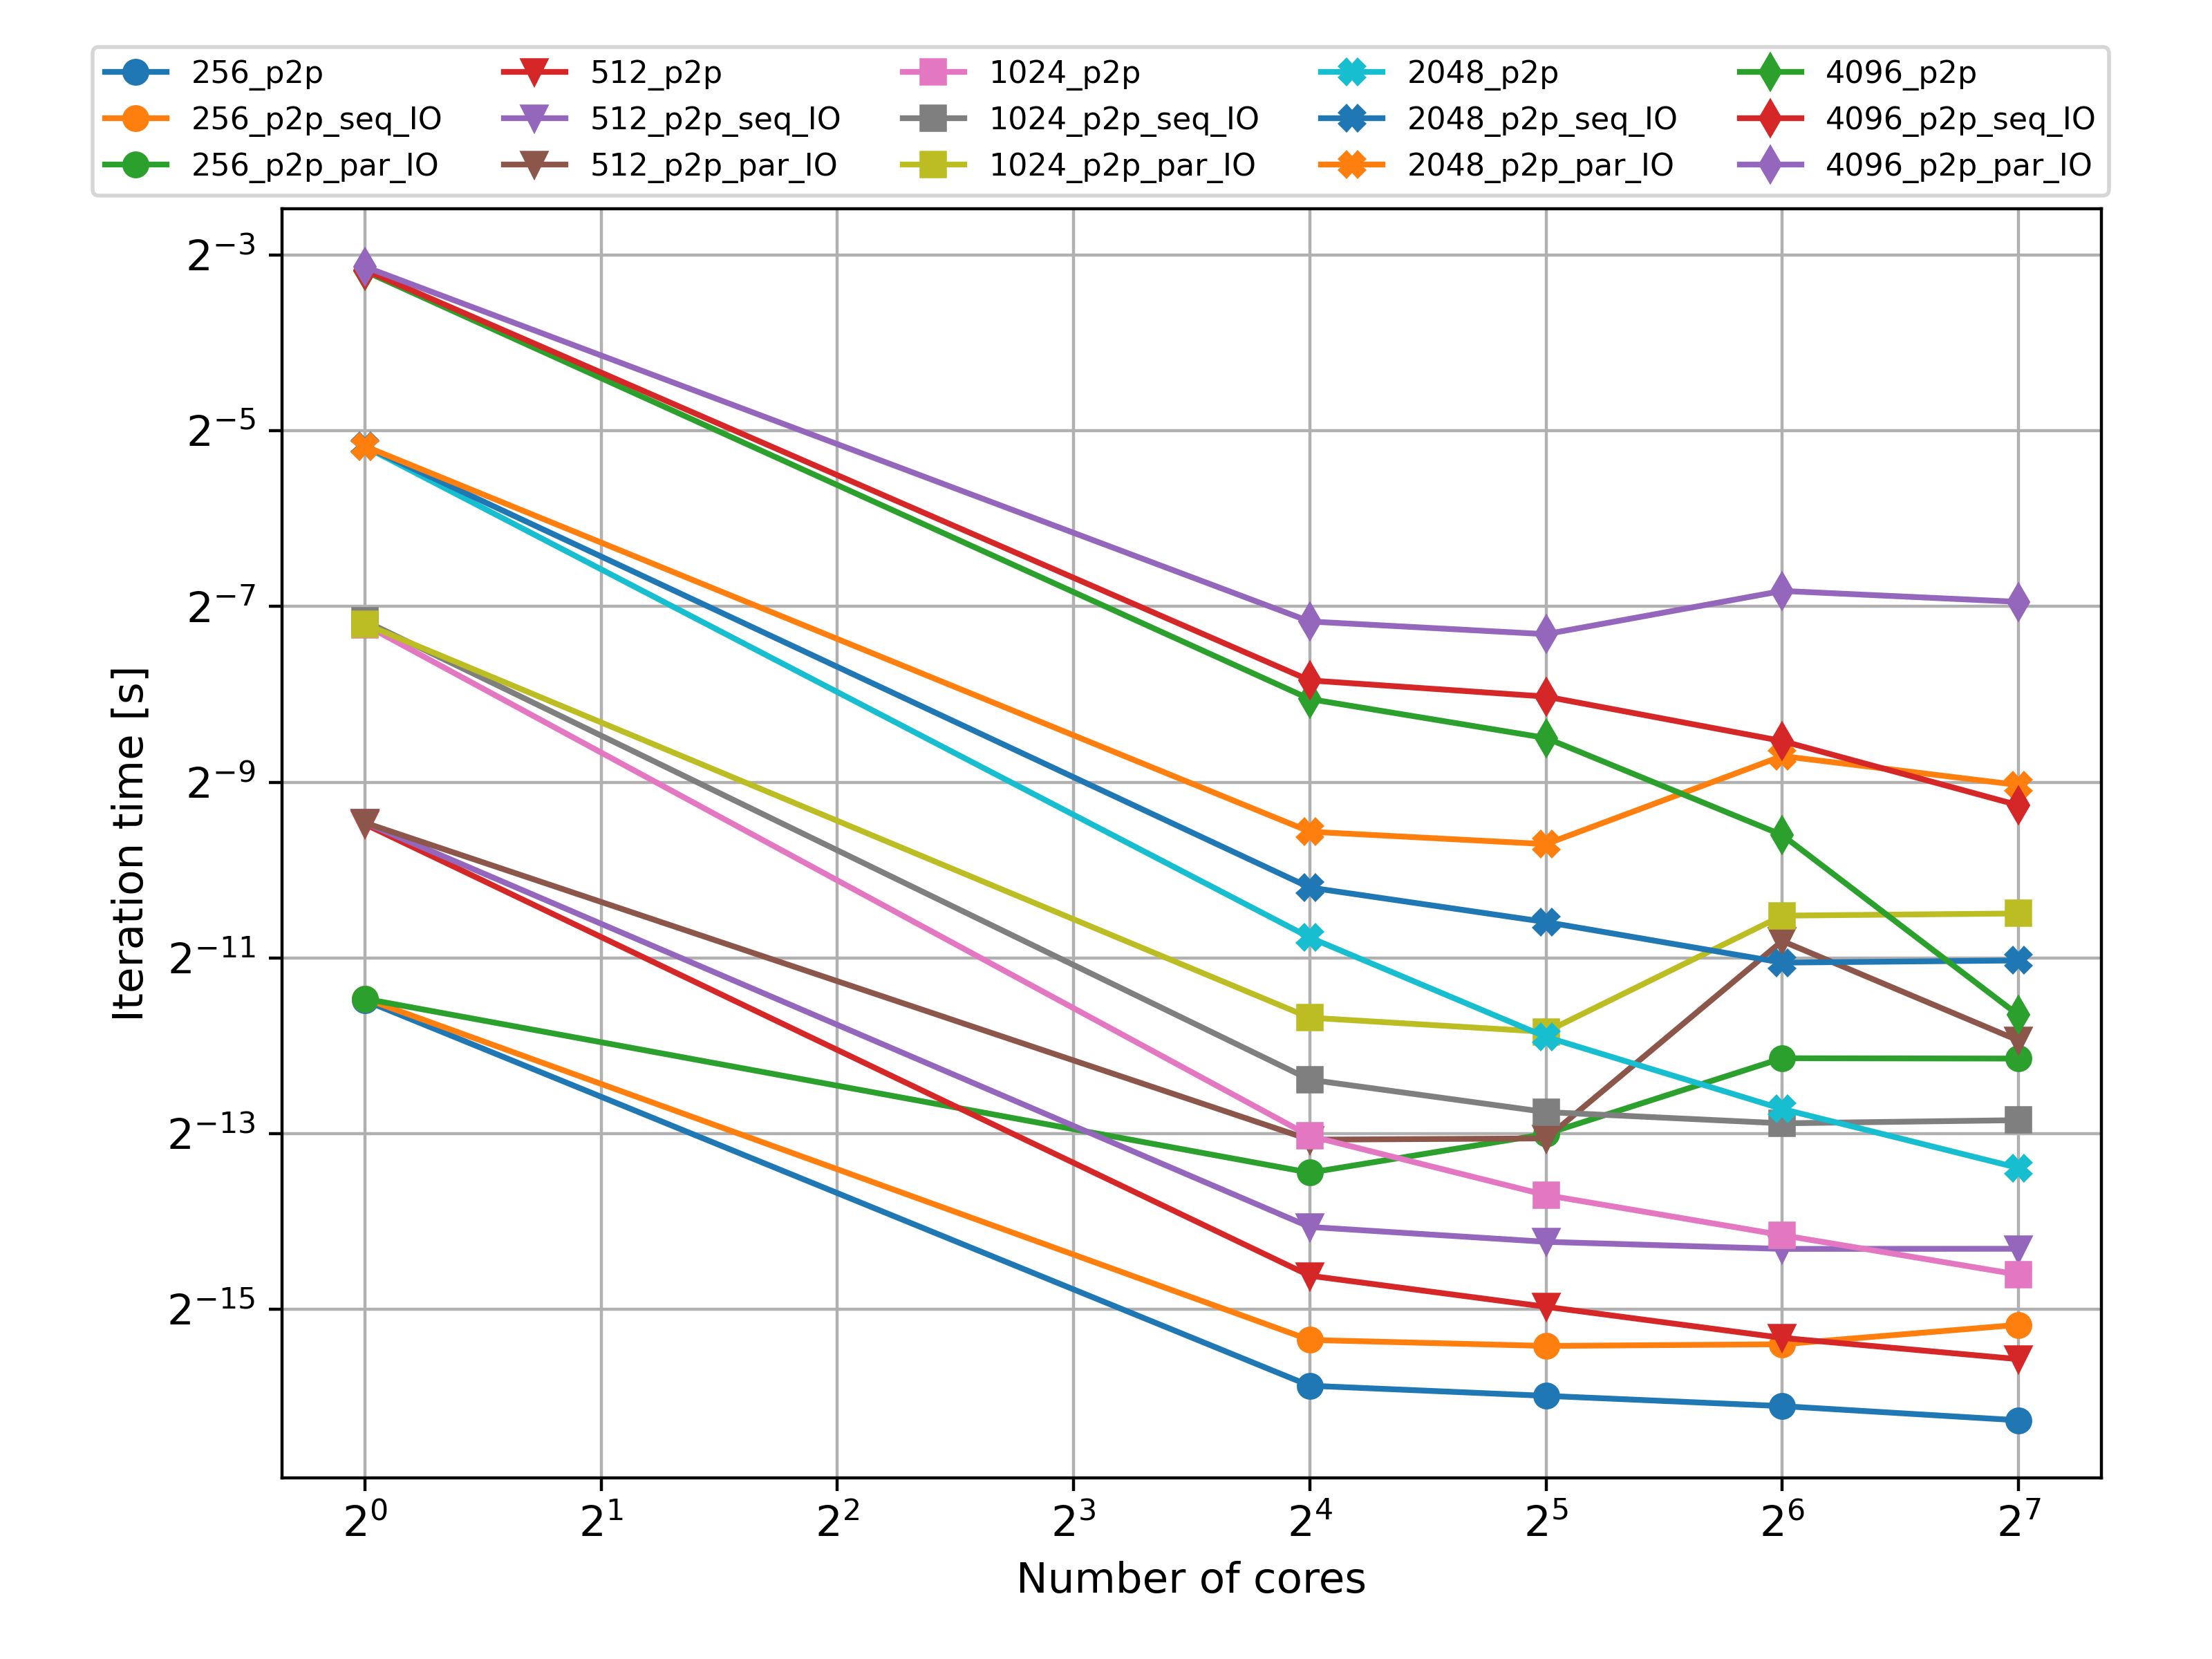
\includegraphics[width=\textwidth]{docs/figures/ppp_scaling_mpi_p2p.png}
        \caption{Cena výpočtu: čisté MPI s 2D dekompozicí, výměna okrajů pomocí P2P.}
        \label{fig:2D_MPI_P2P_cost}
    \end{subfigure}
    \hfill
    \begin{subfigure}{0.45\textwidth}
        \centering
        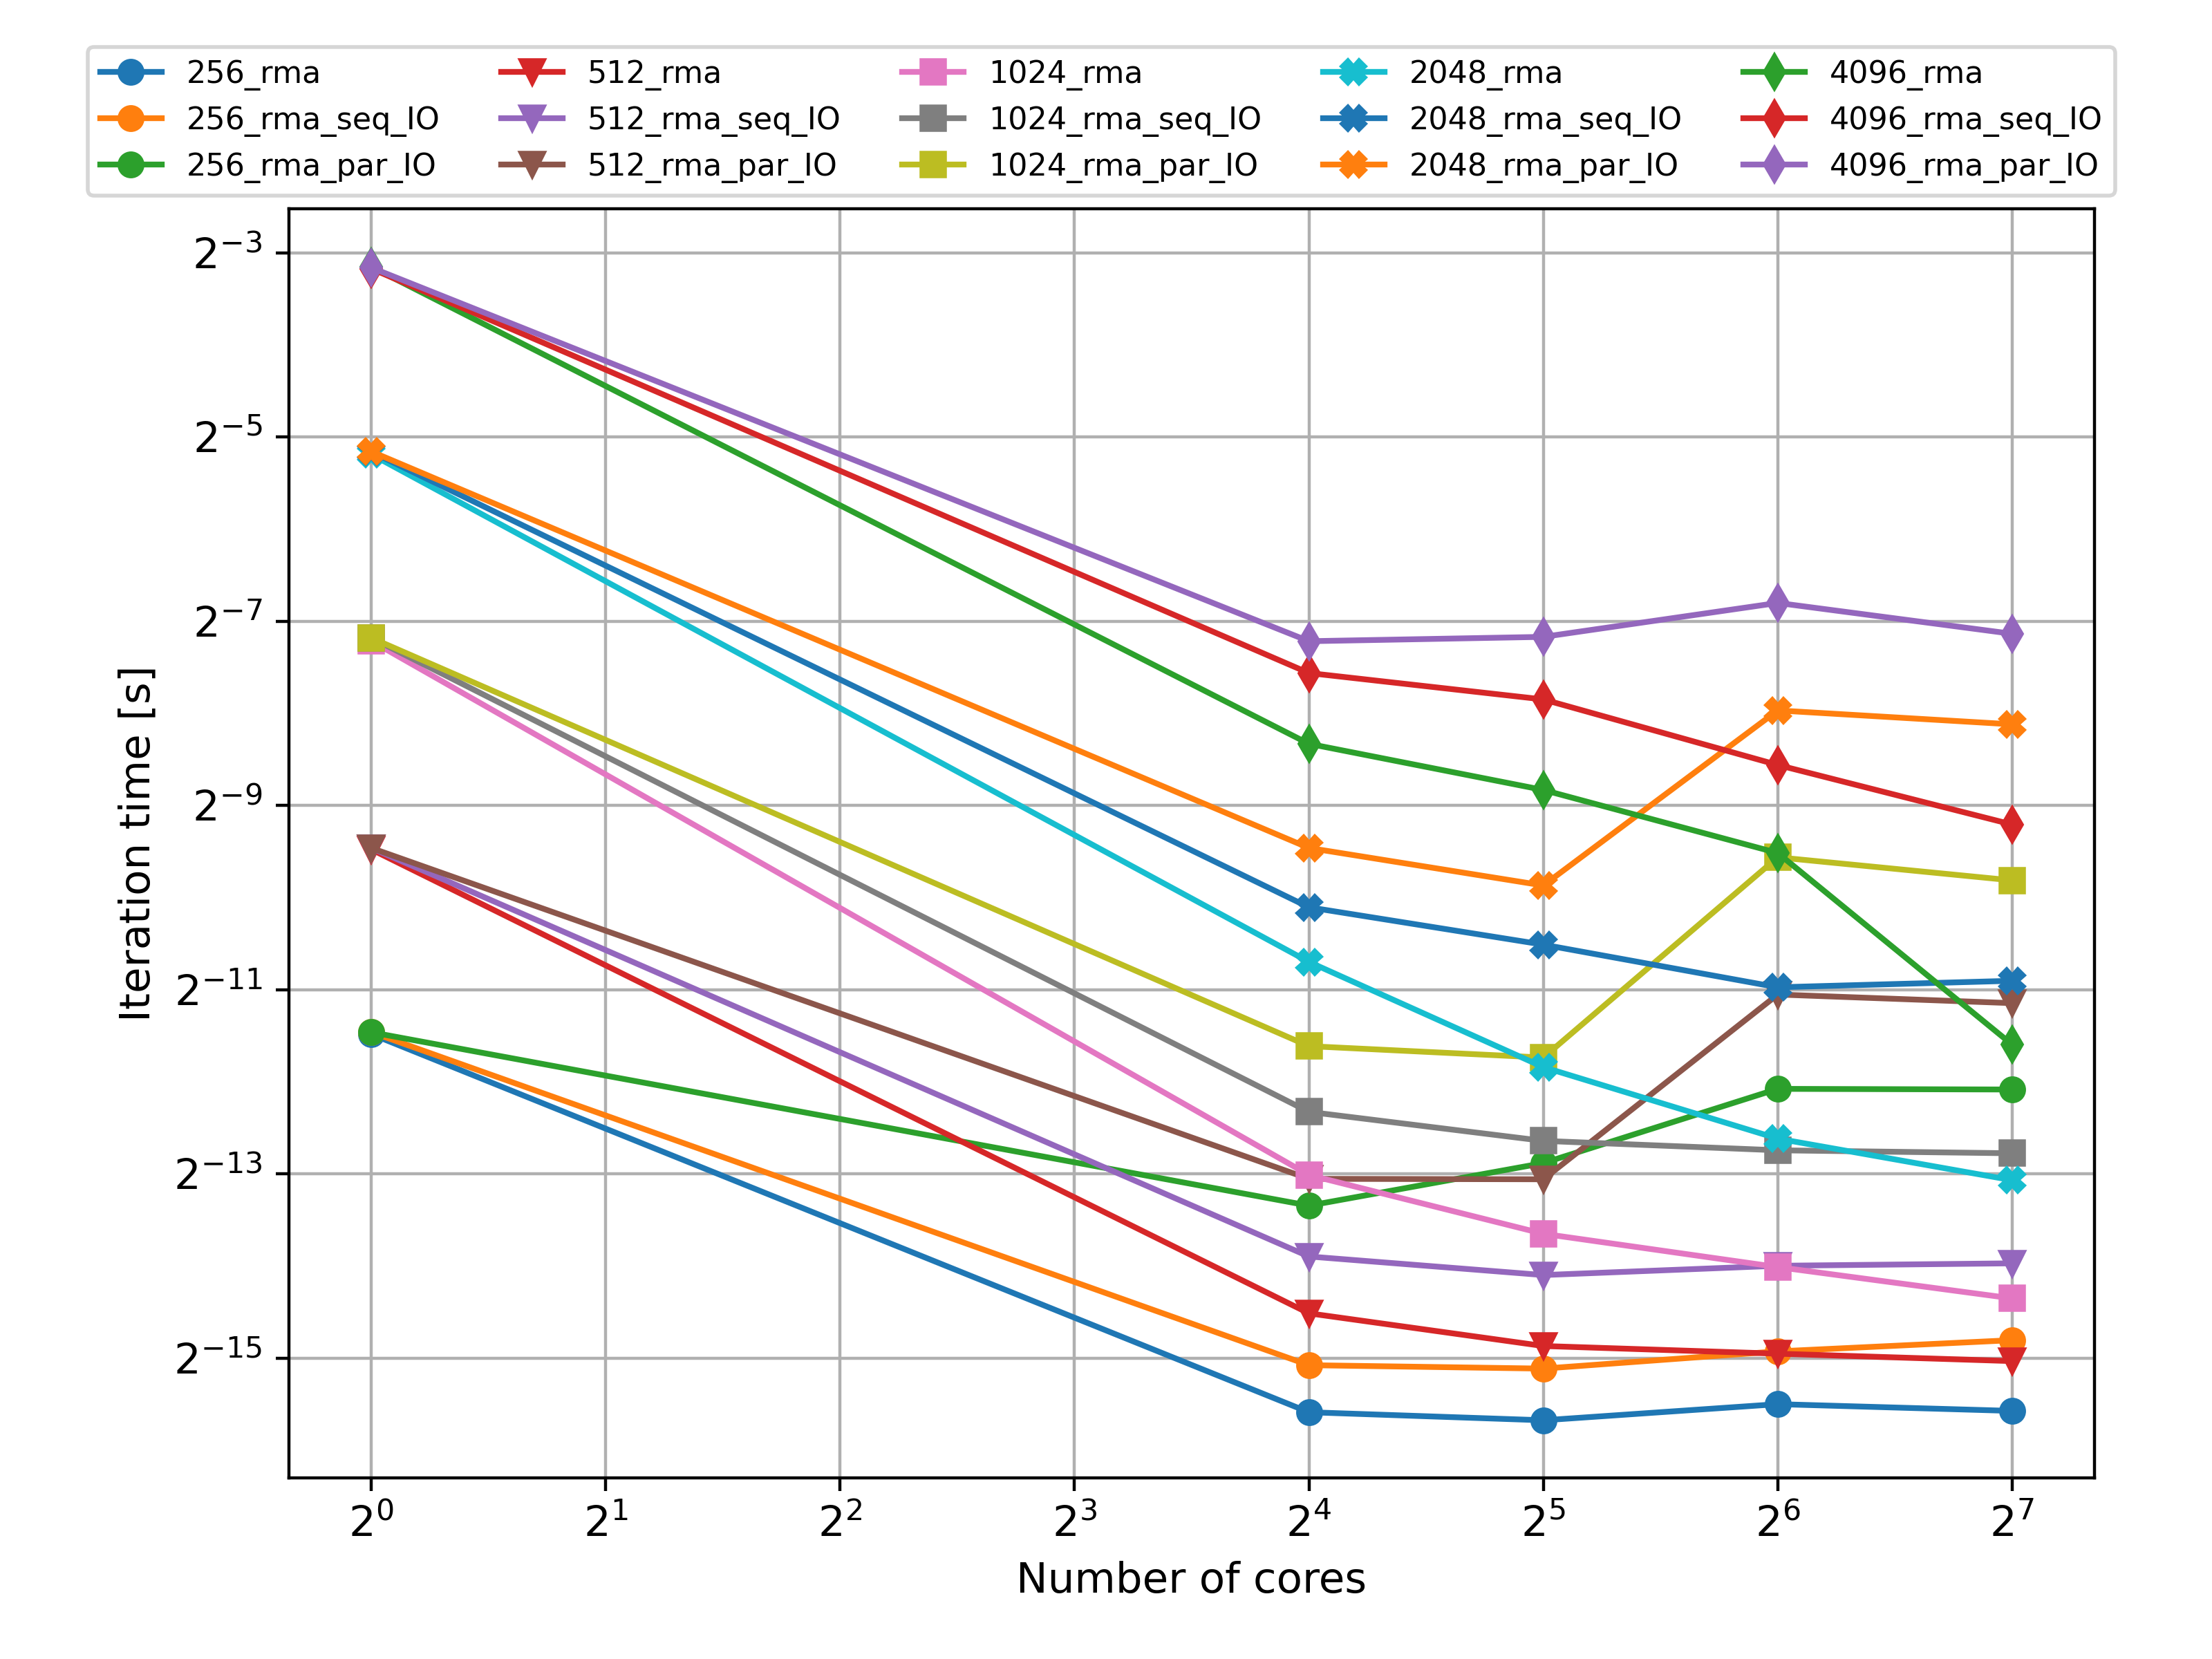
\includegraphics[width=\textwidth]{docs/figures/ppp_scaling_mpi_rma.png}
        \caption{Cena výpočtu: čisté MPI s 2D dekompozicí, výměna okrajů pomocí RMA.}
        \label{fig:2D_MPI_RMA_cost}
    \end{subfigure}
    \caption{Silné škálování a cena výpočtu: čisté MPI s 2D dekompozicí.}
    \label{fig:2D_MPI}
\end{figure}

% ----- Hybrid 2D -----
\begin{figure}[H]
    \centering
    \begin{subfigure}{0.45\textwidth}
        \centering
        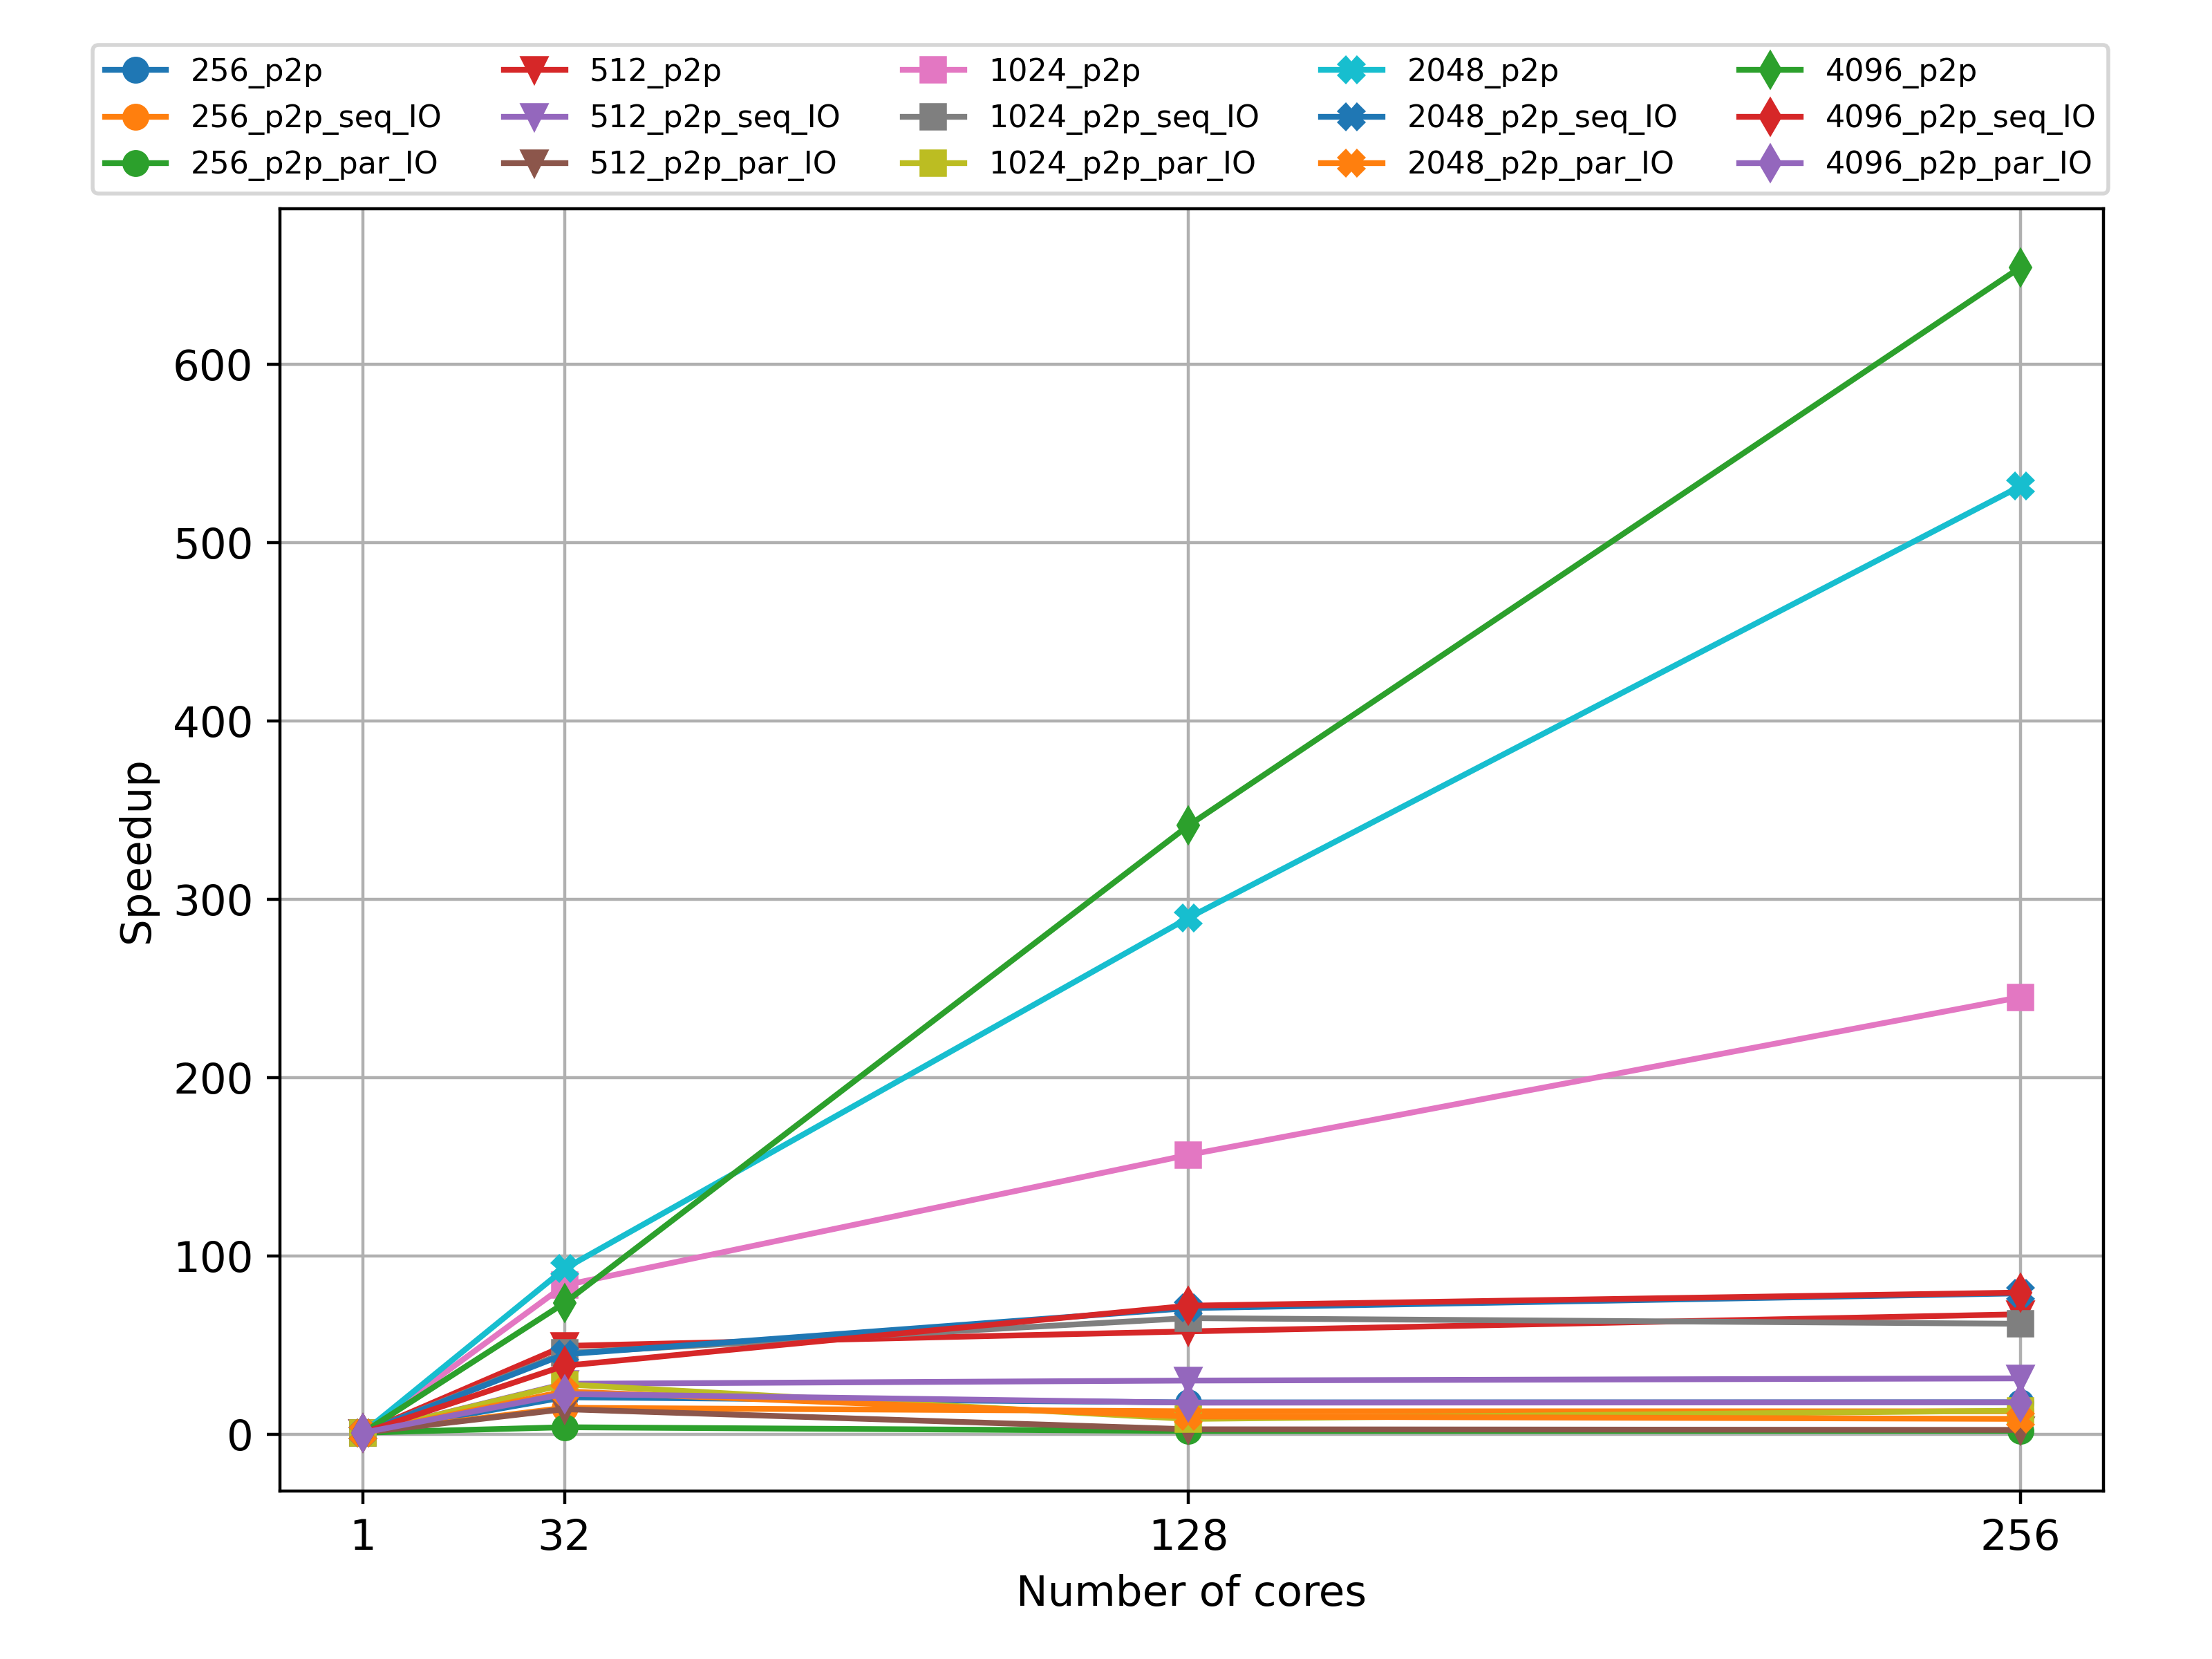
\includegraphics[width=\textwidth]{docs/figures/ppp_speedup_hybrid_p2p.png}
        \caption{Silné škálování: hybridní MPI s 2D dekompozicí, výměna okrajů pomocí P2P.}
        \label{fig:2D_hybrid_P2P}
    \end{subfigure}
    \hfill
    \begin{subfigure}{0.45\textwidth}
        \centering
        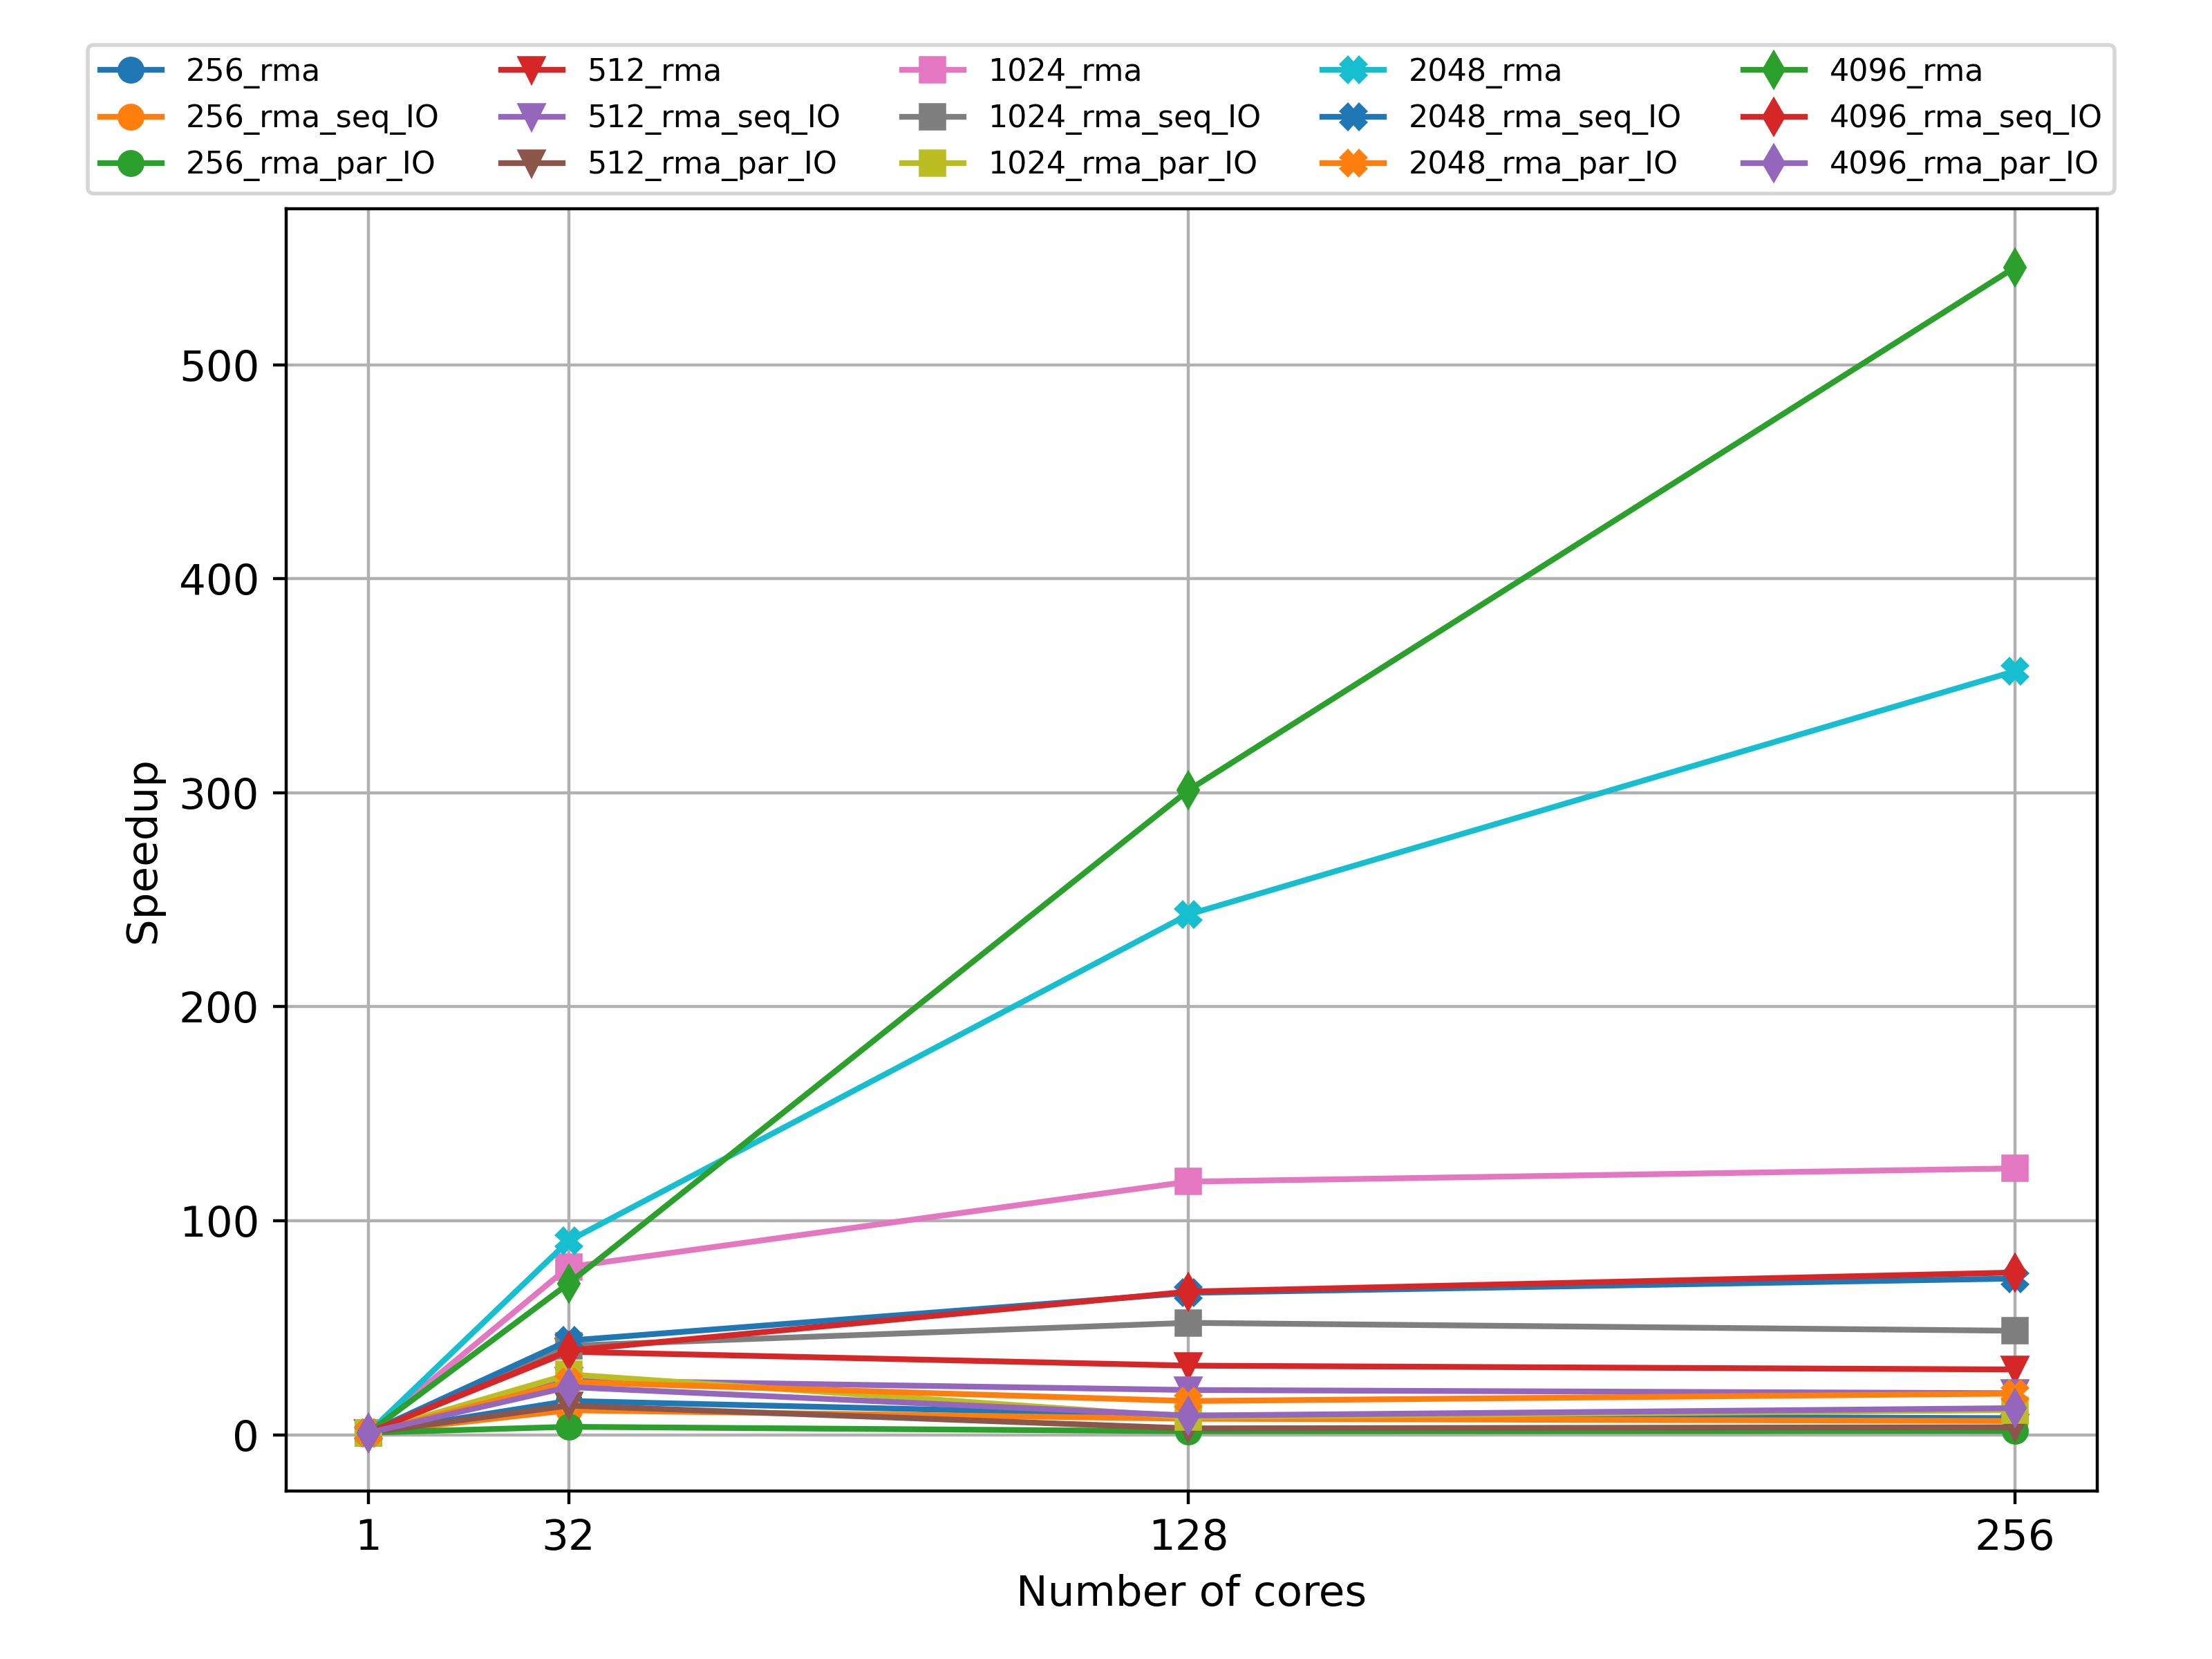
\includegraphics[width=\textwidth]{docs/figures/ppp_speedup_hybrid_rma.png}
        \caption{Silné škálování: hybridní MPI s 2D dekompozicí, výměna okrajů pomocí RMA.}
        \label{fig:2D_hybrid_RMA}
    \end{subfigure}

    \begin{subfigure}{0.45\textwidth}
        \centering
        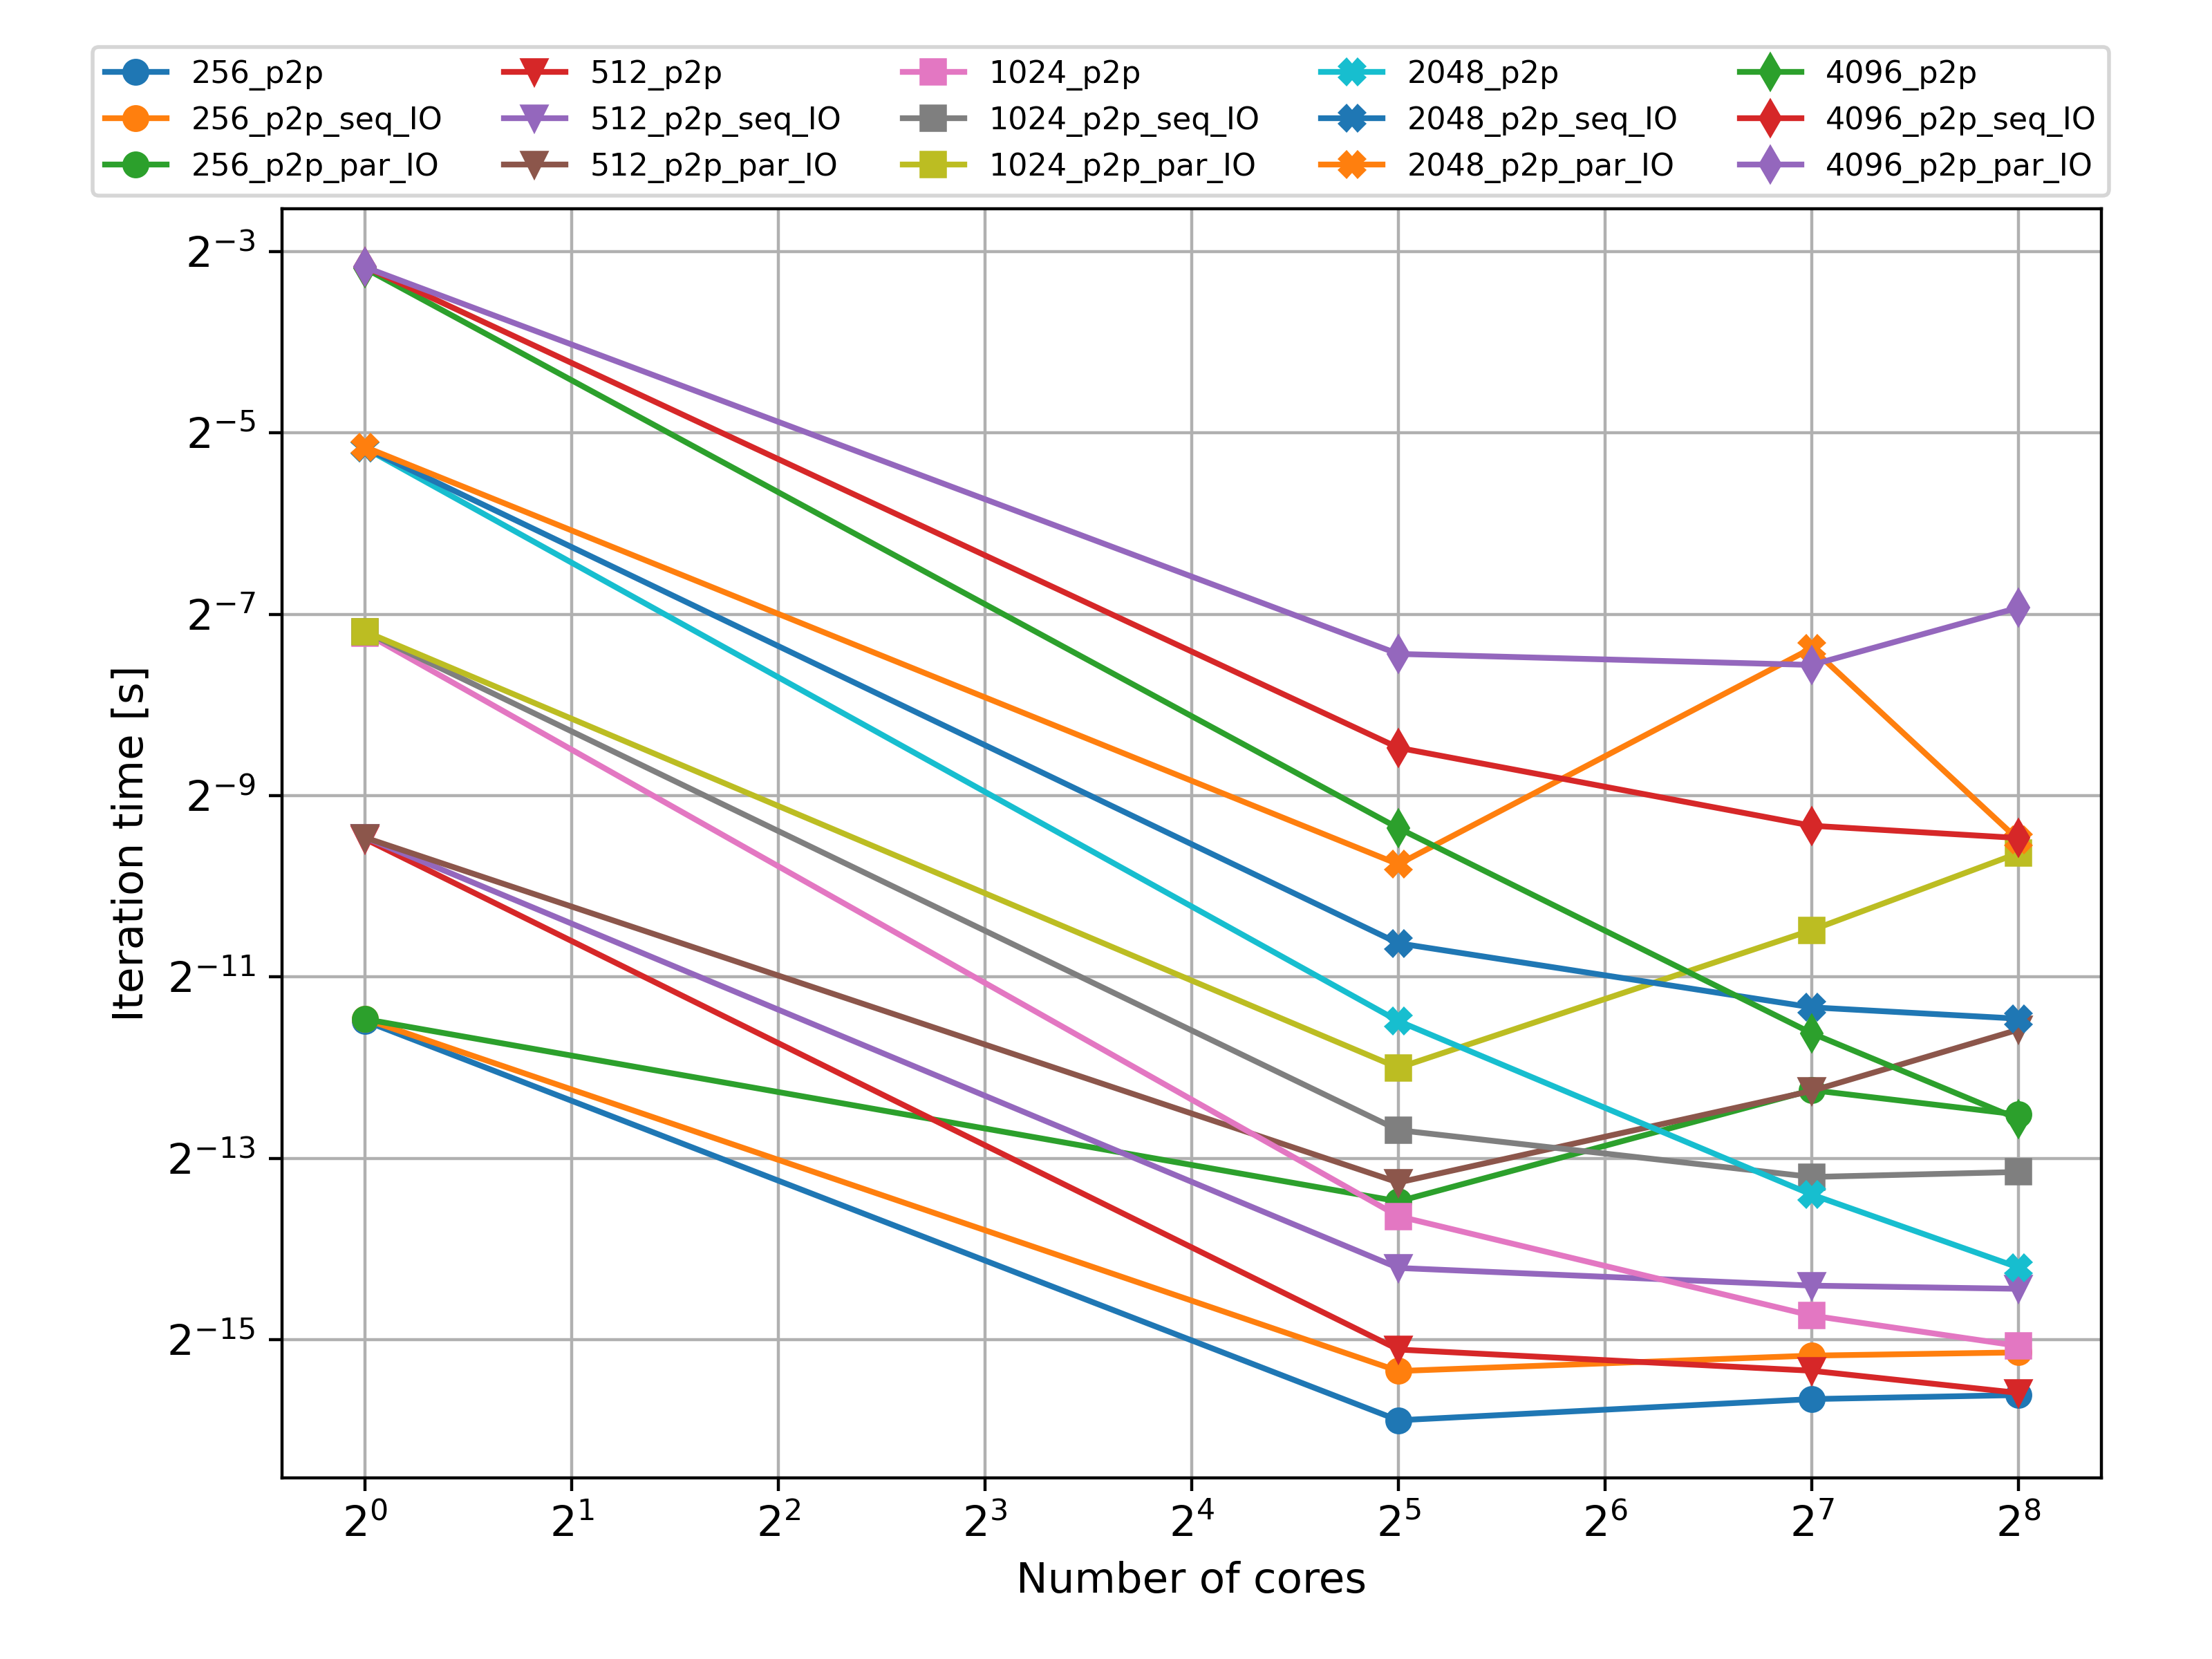
\includegraphics[width=\textwidth]{docs/figures/ppp_scaling_hybrid_p2p.png}
        \caption{Cena výpočtu: hybridní MPI s 2D dekompozicí, výměna okrajů pomocí P2P.}
        \label{fig:2D_hybrid_P2P_cost}
    \end{subfigure}
    \hfill
    \begin{subfigure}{0.45\textwidth}
        \centering
        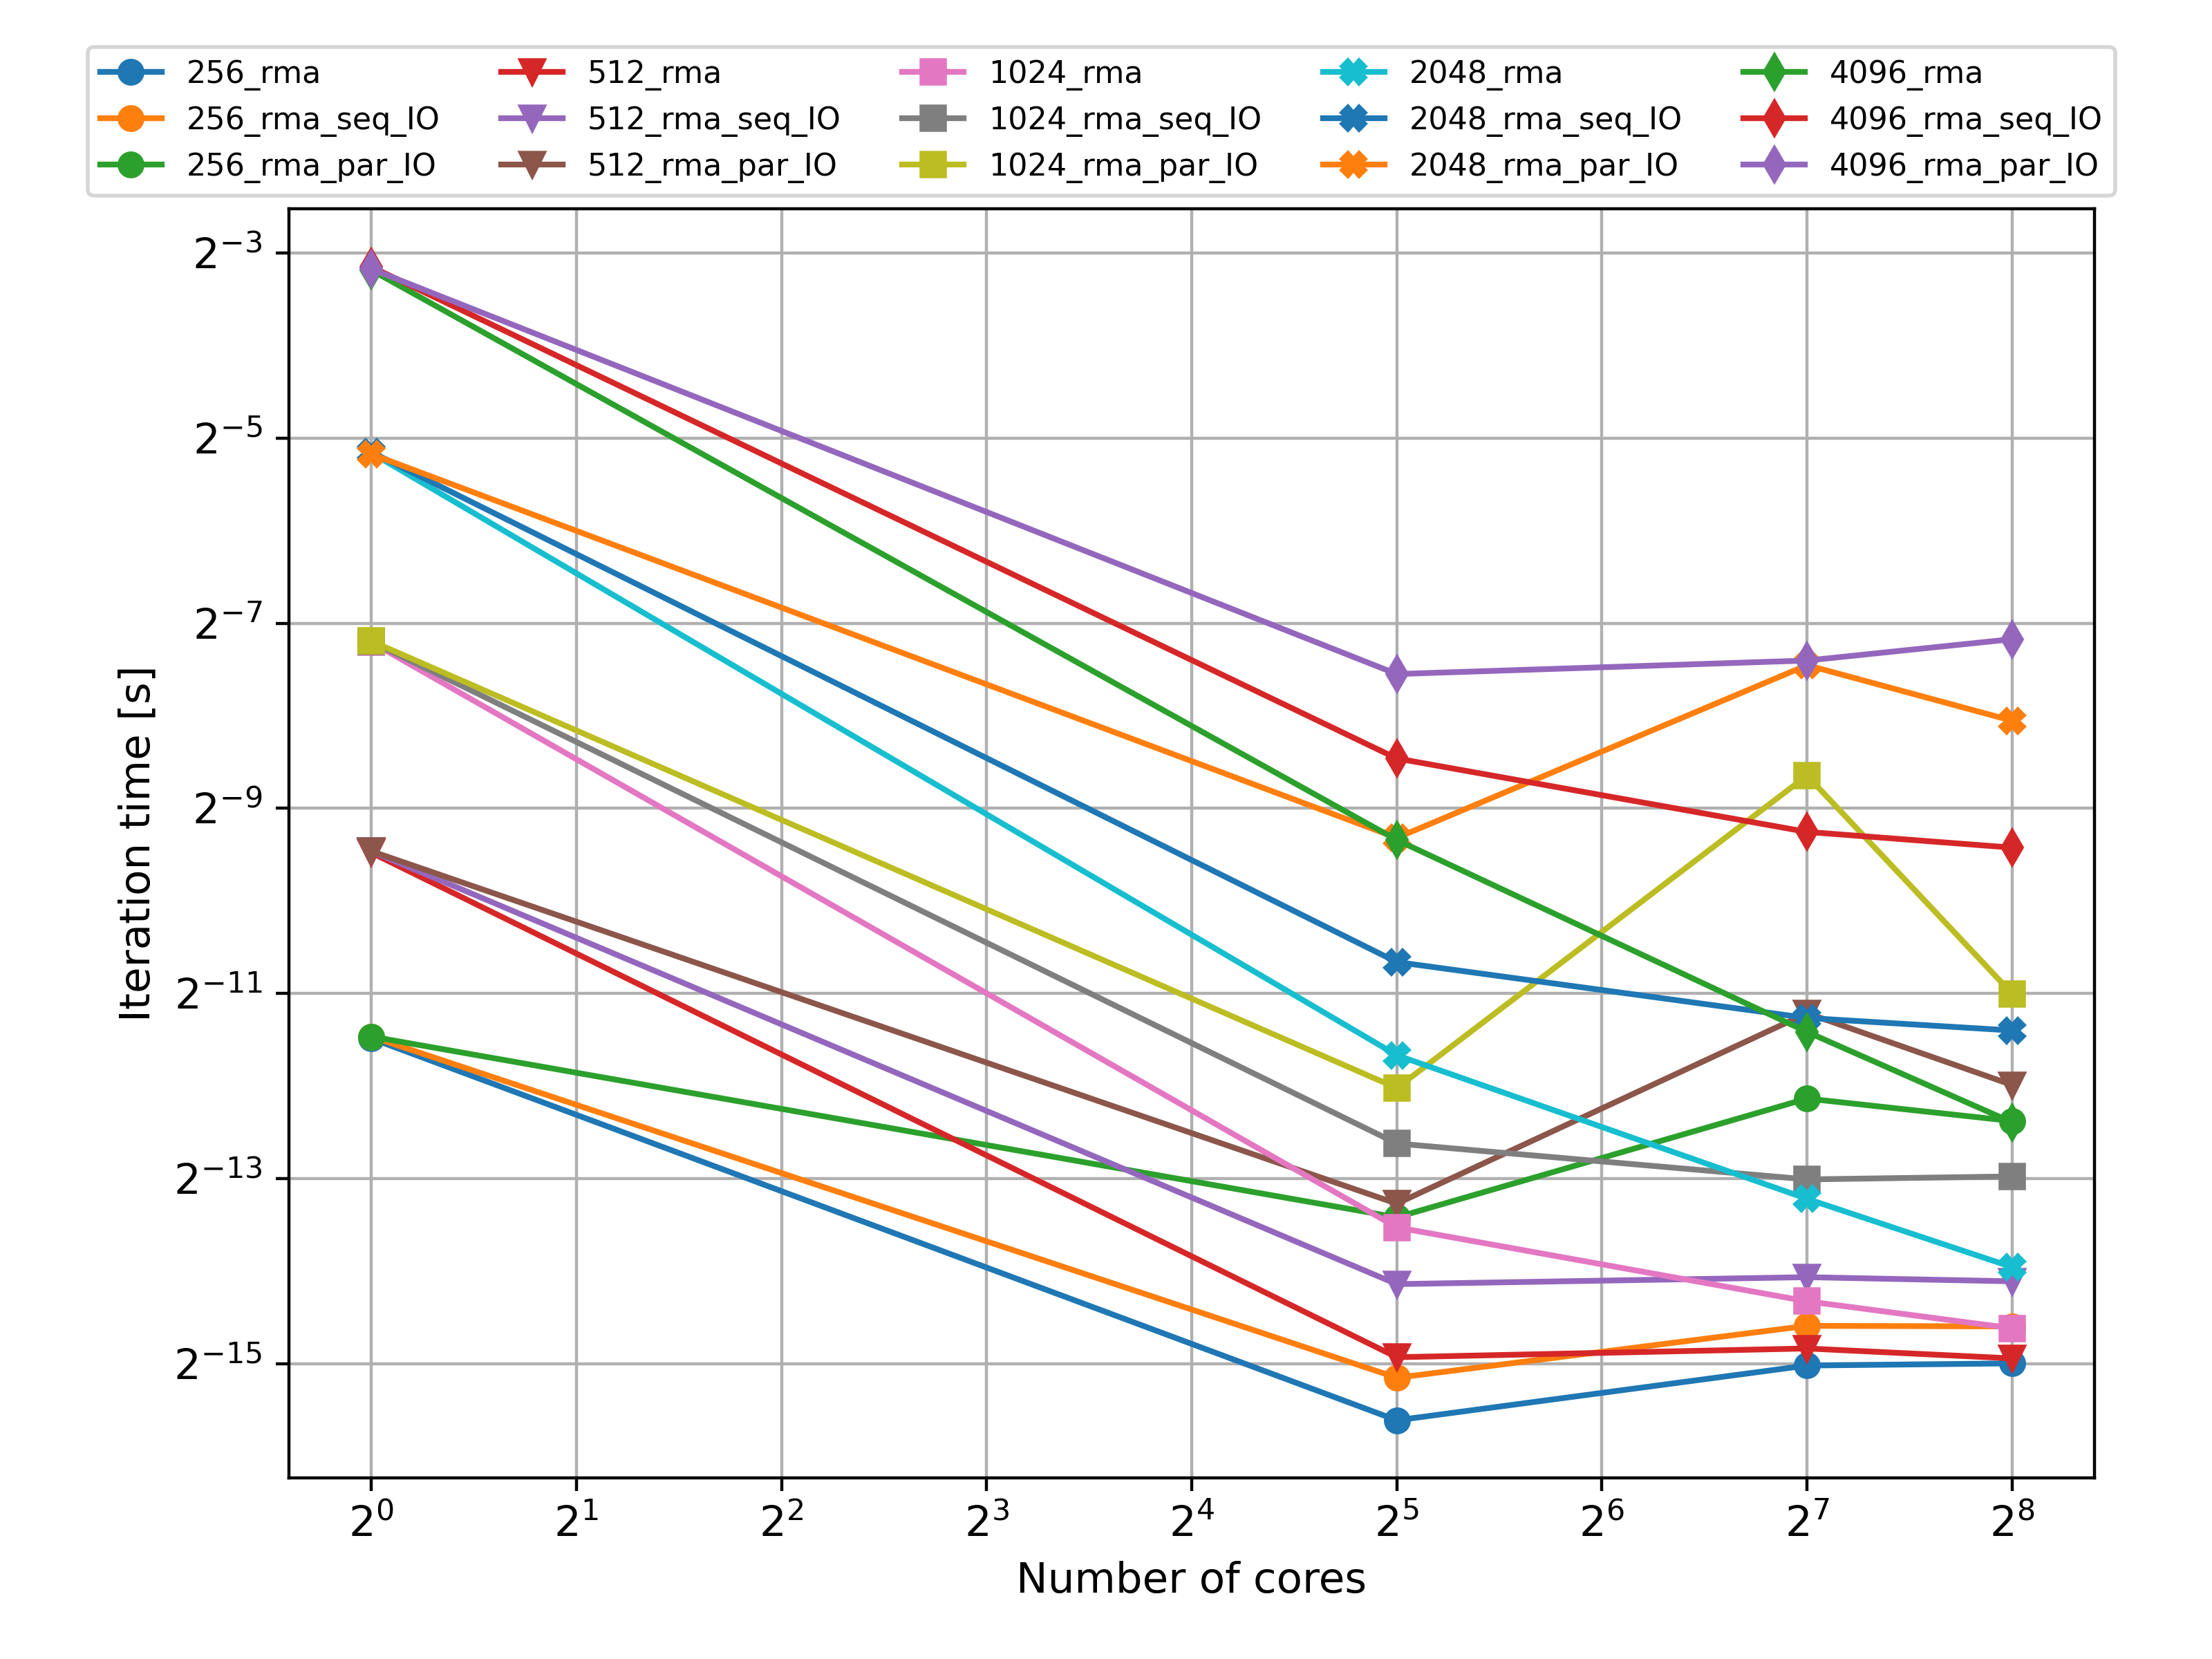
\includegraphics[width=\textwidth]{docs/figures/ppp_scaling_hybrid_rma.png}
        \caption{Cena výpočtu: hybridní MPI s 2D dekompozicí, výměna okrajů pomocí RMA.}
        \label{fig:2D_hybrid_RMA_cost}
    \end{subfigure}
    \caption{Silné škálování a cena výpočtu: hybridní MPI s 2D dekompozicí.}
    \label{fig:2D_hybrid}
\end{figure}

% ----- Hybrid 1D -----
\begin{figure}[H]
    \centering
    \begin{subfigure}{0.45\textwidth}
        \centering
        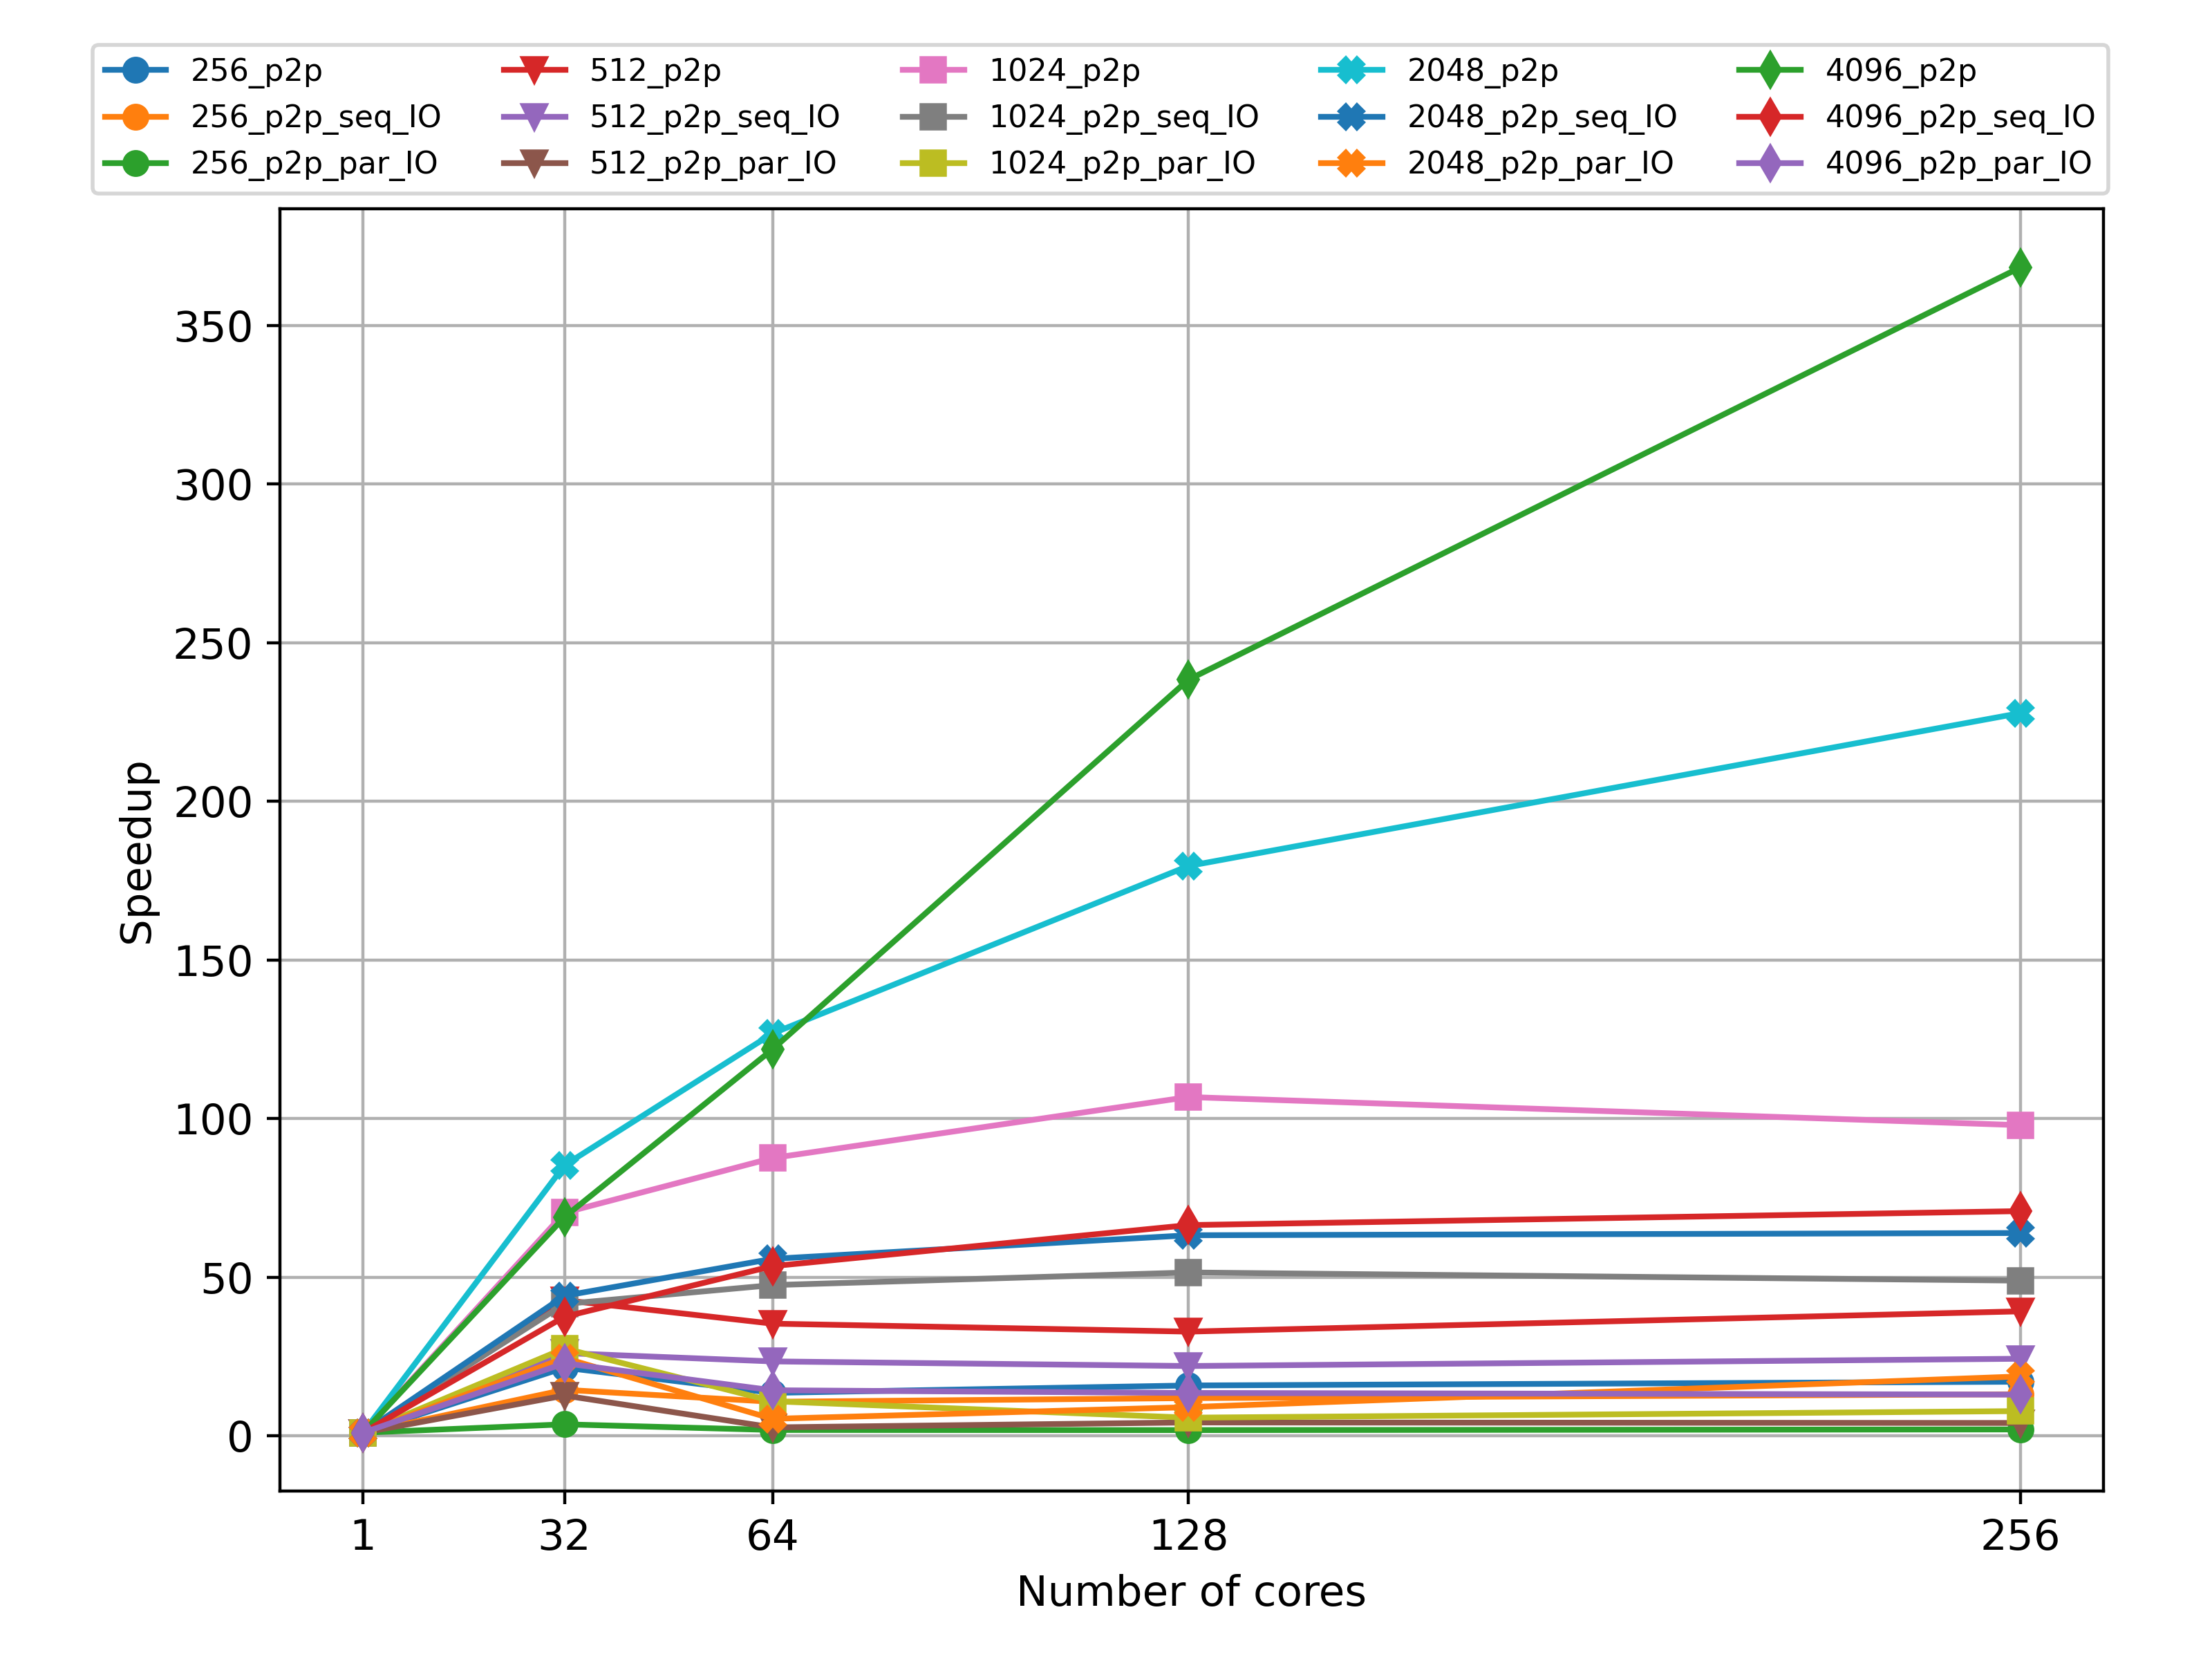
\includegraphics[width=\textwidth]{docs/figures/ppp_speedup_hybrid_1D_p2p.png}
        \caption{Silné škálování: hybridní MPI s 1D dekompozicí, výměna okrajů pomocí P2P.}
        \label{fig:1D_hybrid_P2P}
    \end{subfigure}
    \hfill
    \begin{subfigure}{0.45\textwidth}
        \centering
        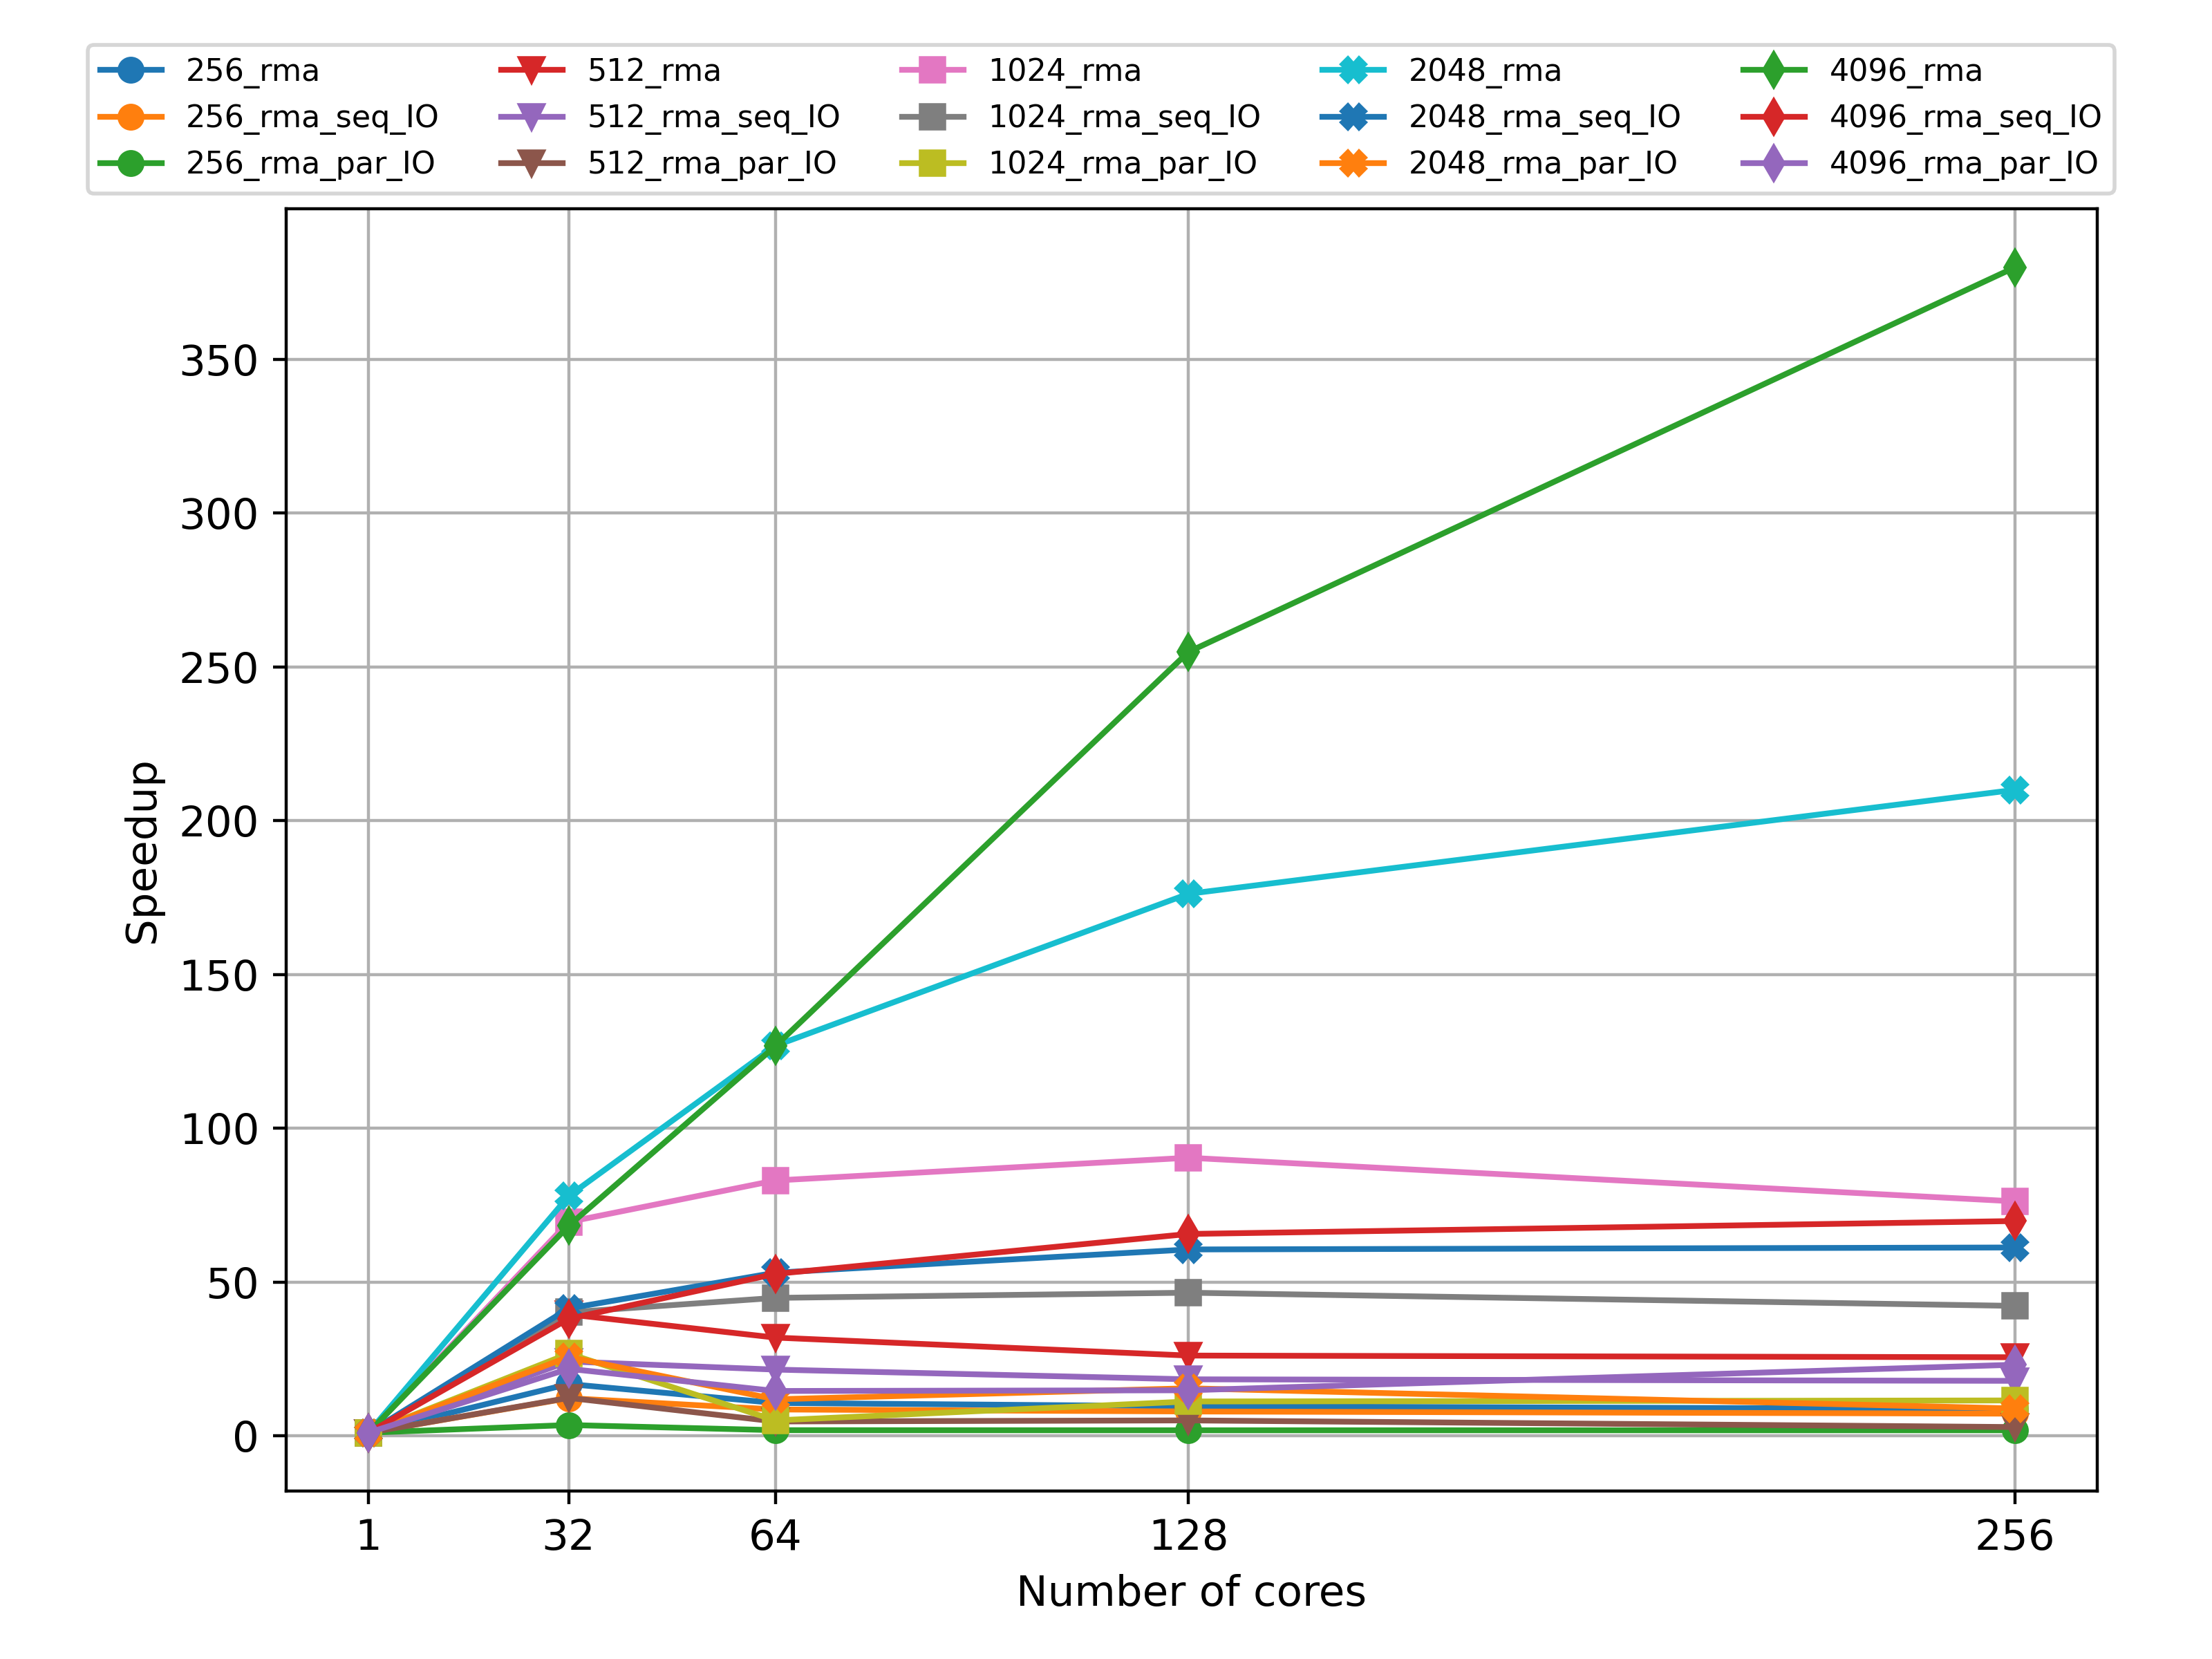
\includegraphics[width=\textwidth]{docs/figures/ppp_speedup_hybrid_1D_rma.png}
        \caption{Silné škálování: hybridní MPI s 1D dekompozicí, výměna okrajů pomocí RMA.}
        \label{fig:1D_hybrid_RMA}
    \end{subfigure}

    \begin{subfigure}{0.45\textwidth}
        \centering
        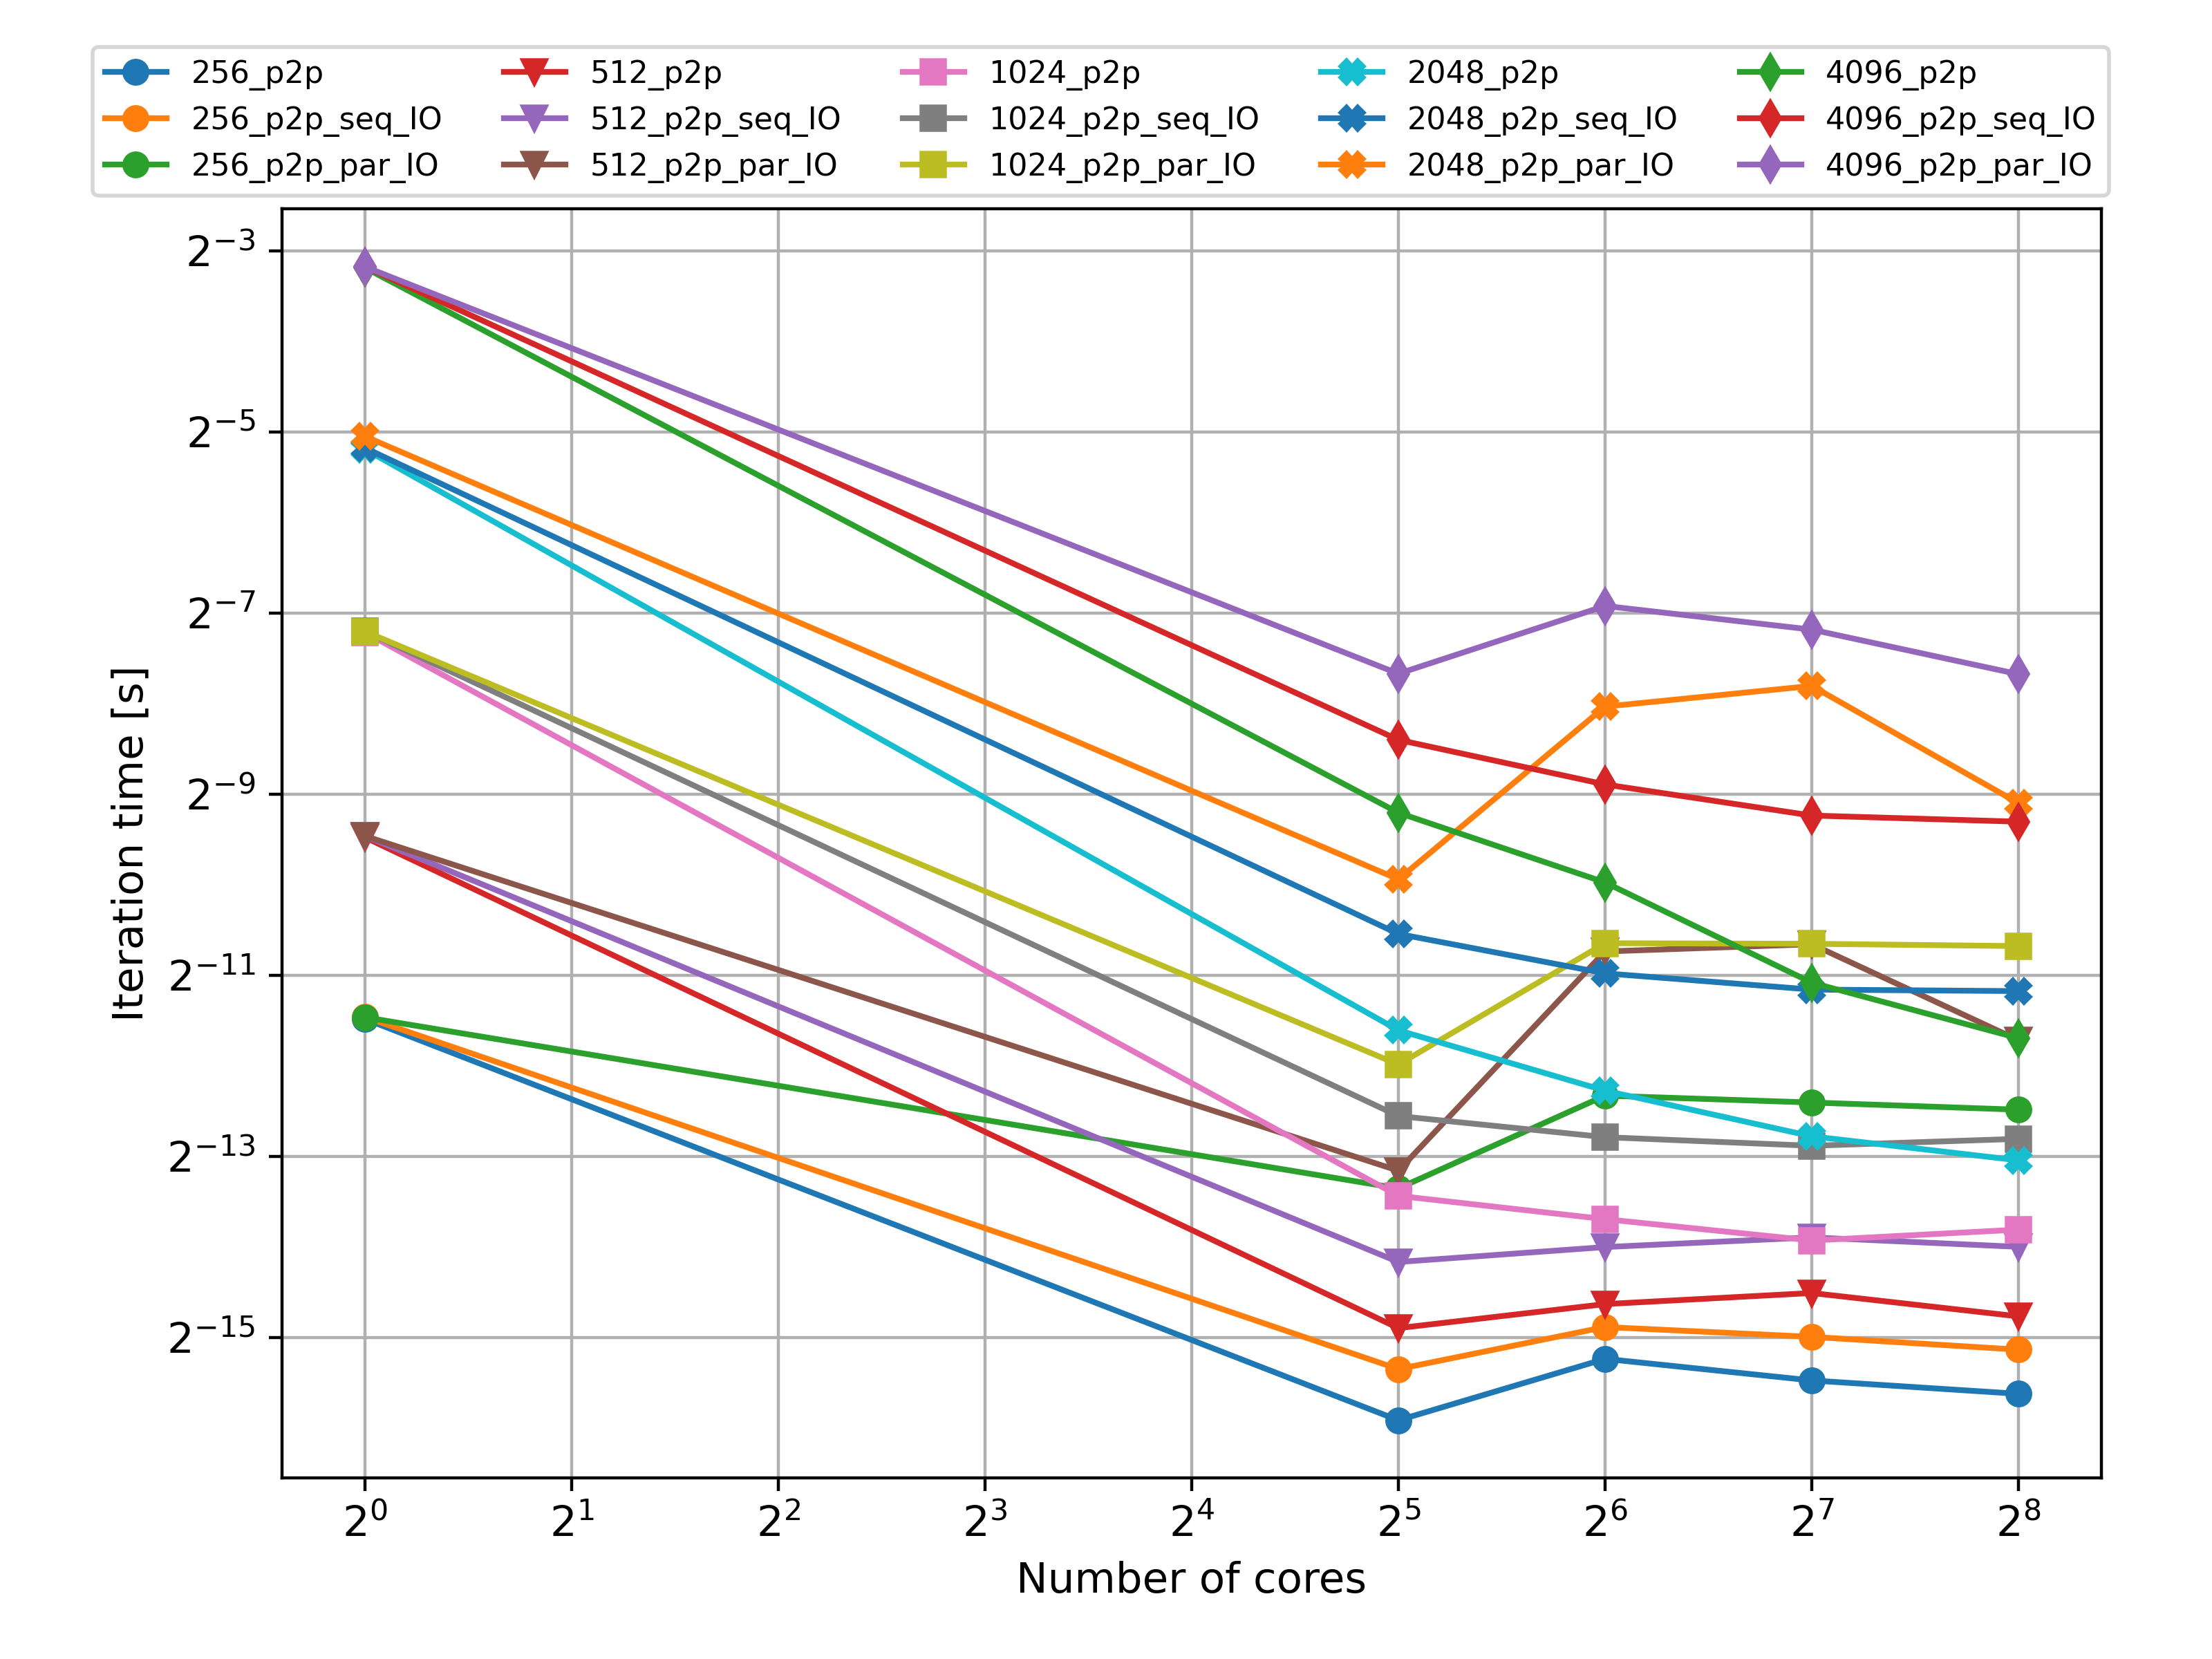
\includegraphics[width=\textwidth]{docs/figures/ppp_scaling_hybrid_1D_p2p.png}
        \caption{Cena výpočtu: hybridní MPI s 1D dekompozicí, výměna okrajů pomocí P2P.}
        \label{fig:1D_hybrid_P2P_cost}
    \end{subfigure}
    \hfill
    \begin{subfigure}{0.45\textwidth}
        \centering
        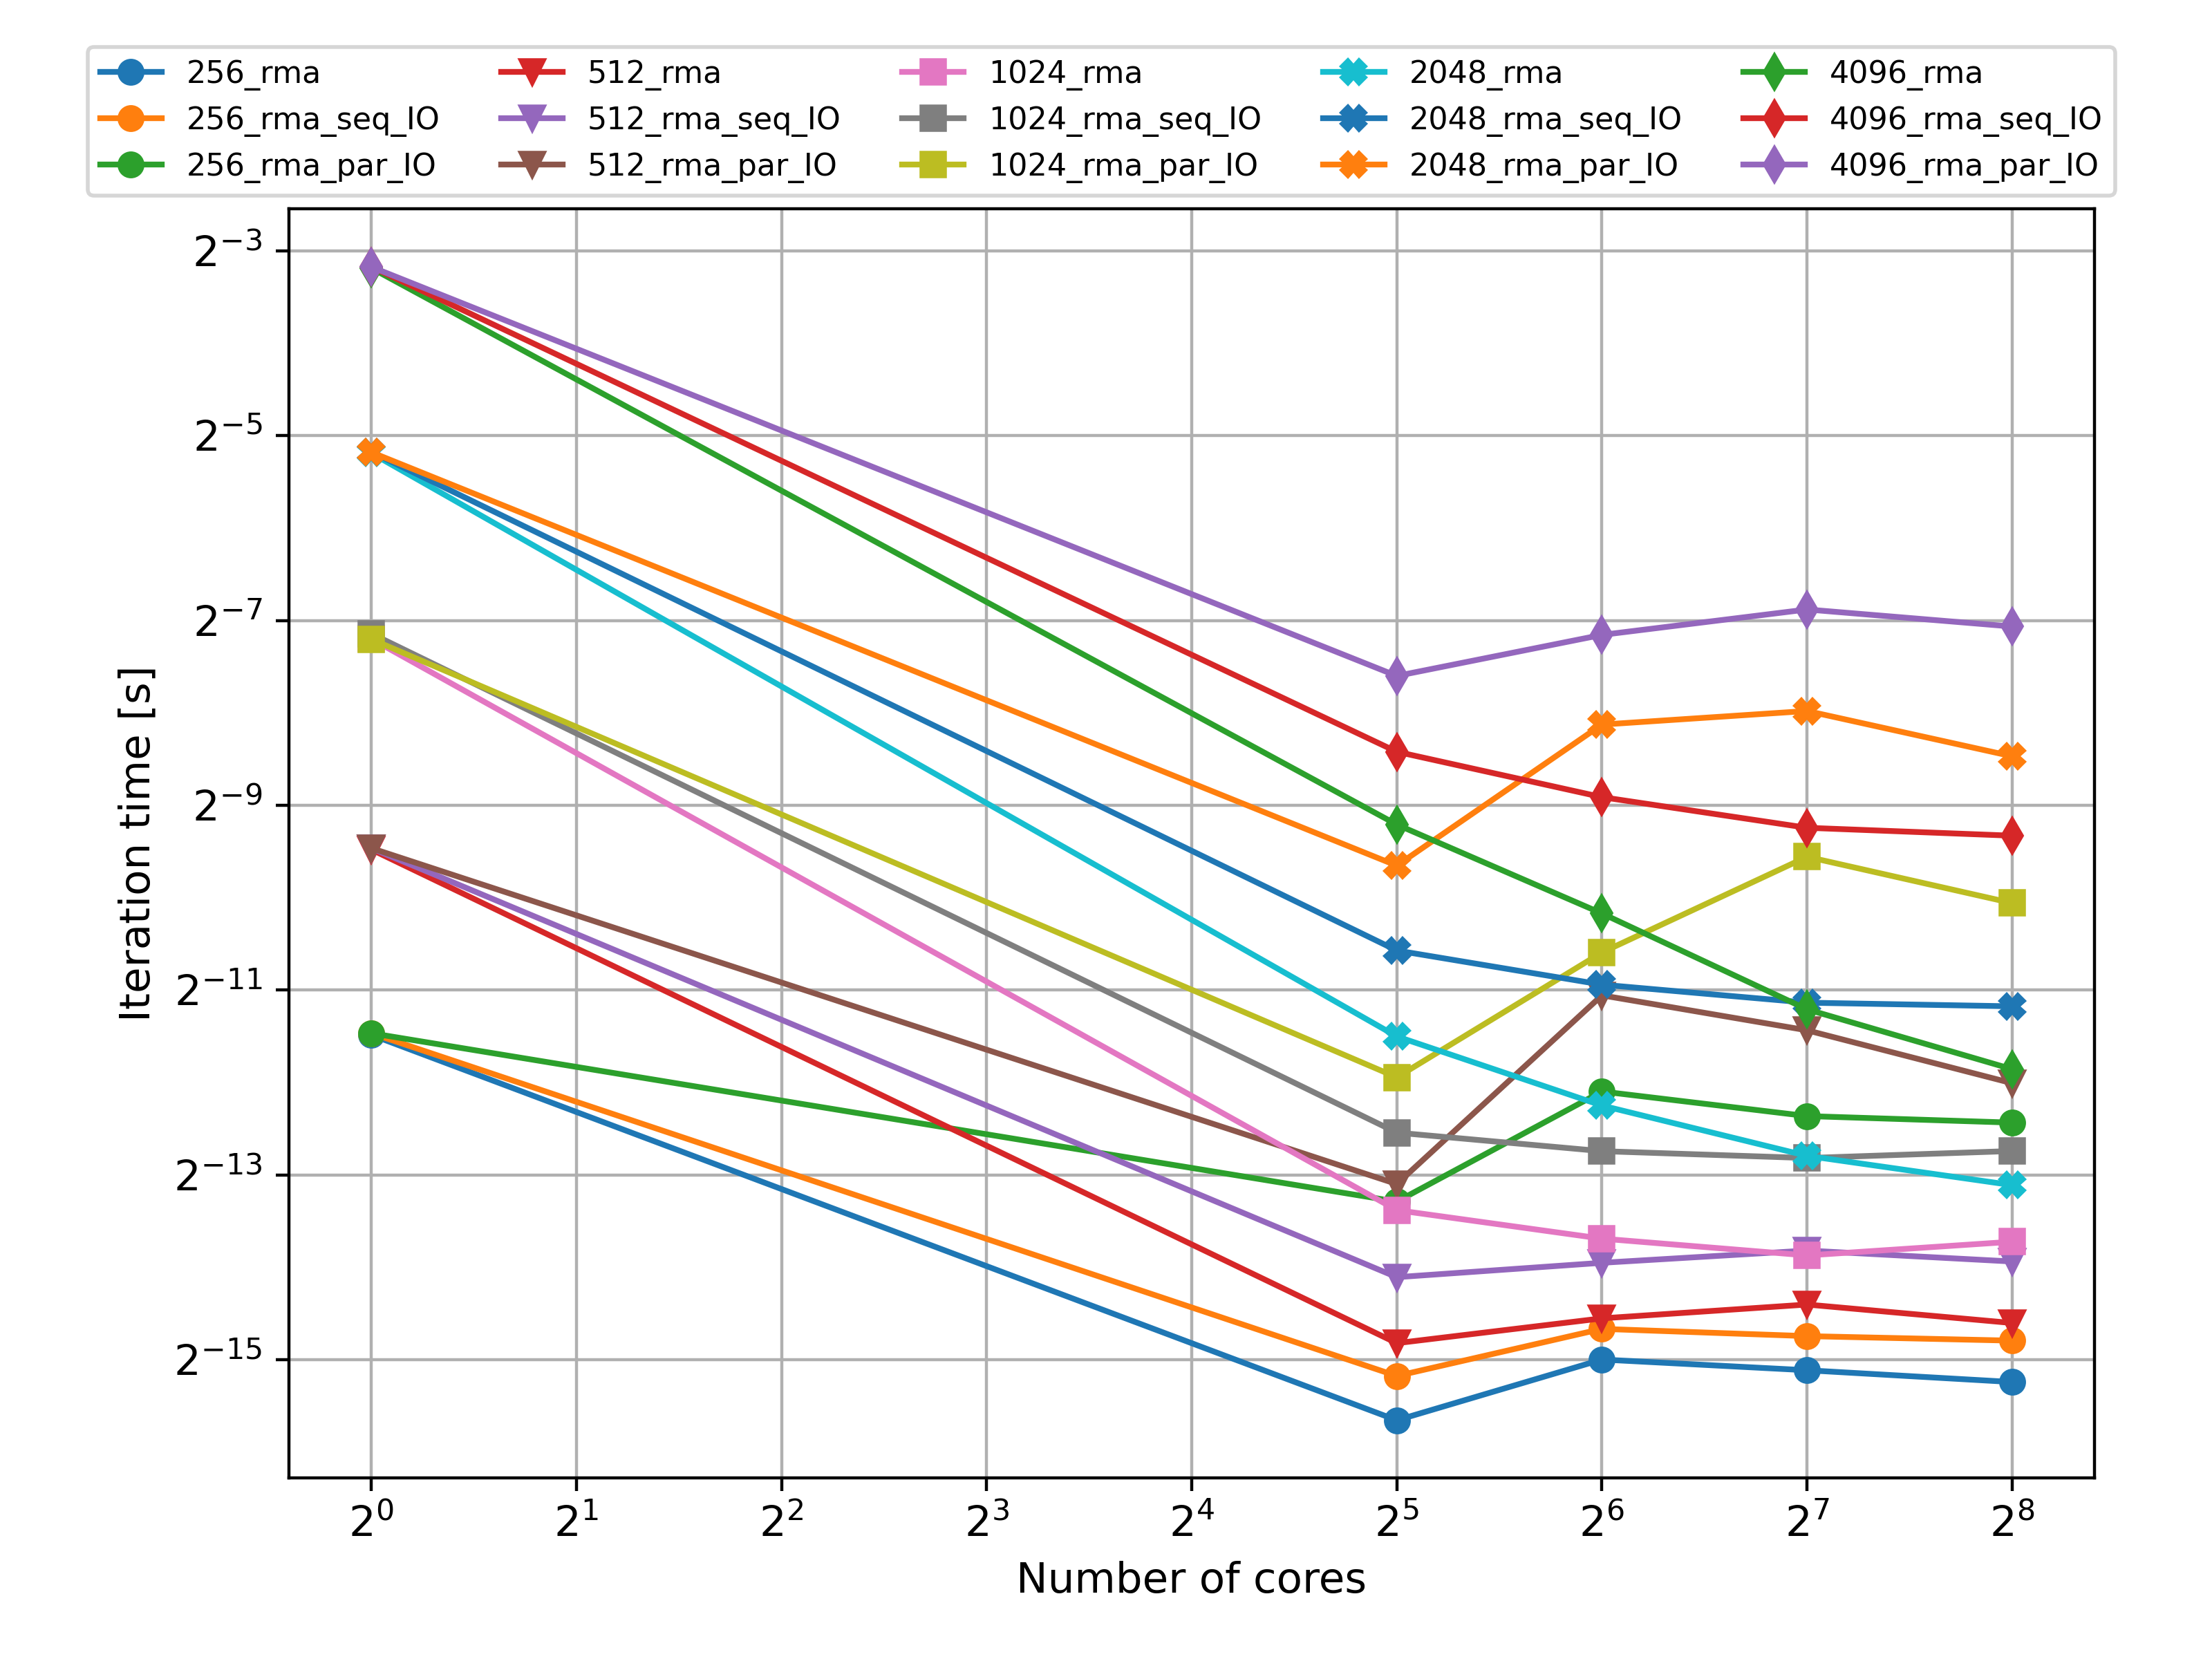
\includegraphics[width=\textwidth]{docs/figures/ppp_scaling_hybrid_1D_rma.png}
        \caption{Cena výpočtu: hybridní MPI s 1D dekompozicí, výměna okrajů pomocí RMA.}
        \label{fig:1D_hybrid_RMA_cost}
    \end{subfigure}
    \caption{Silné škálování a cena výpočtu: hybridní MPI s 1D dekompozicí.}
    \label{fig:1D_hybrid}
\end{figure}

% ----- Weak scaling -----
\begin{figure}[H]
    \centering
    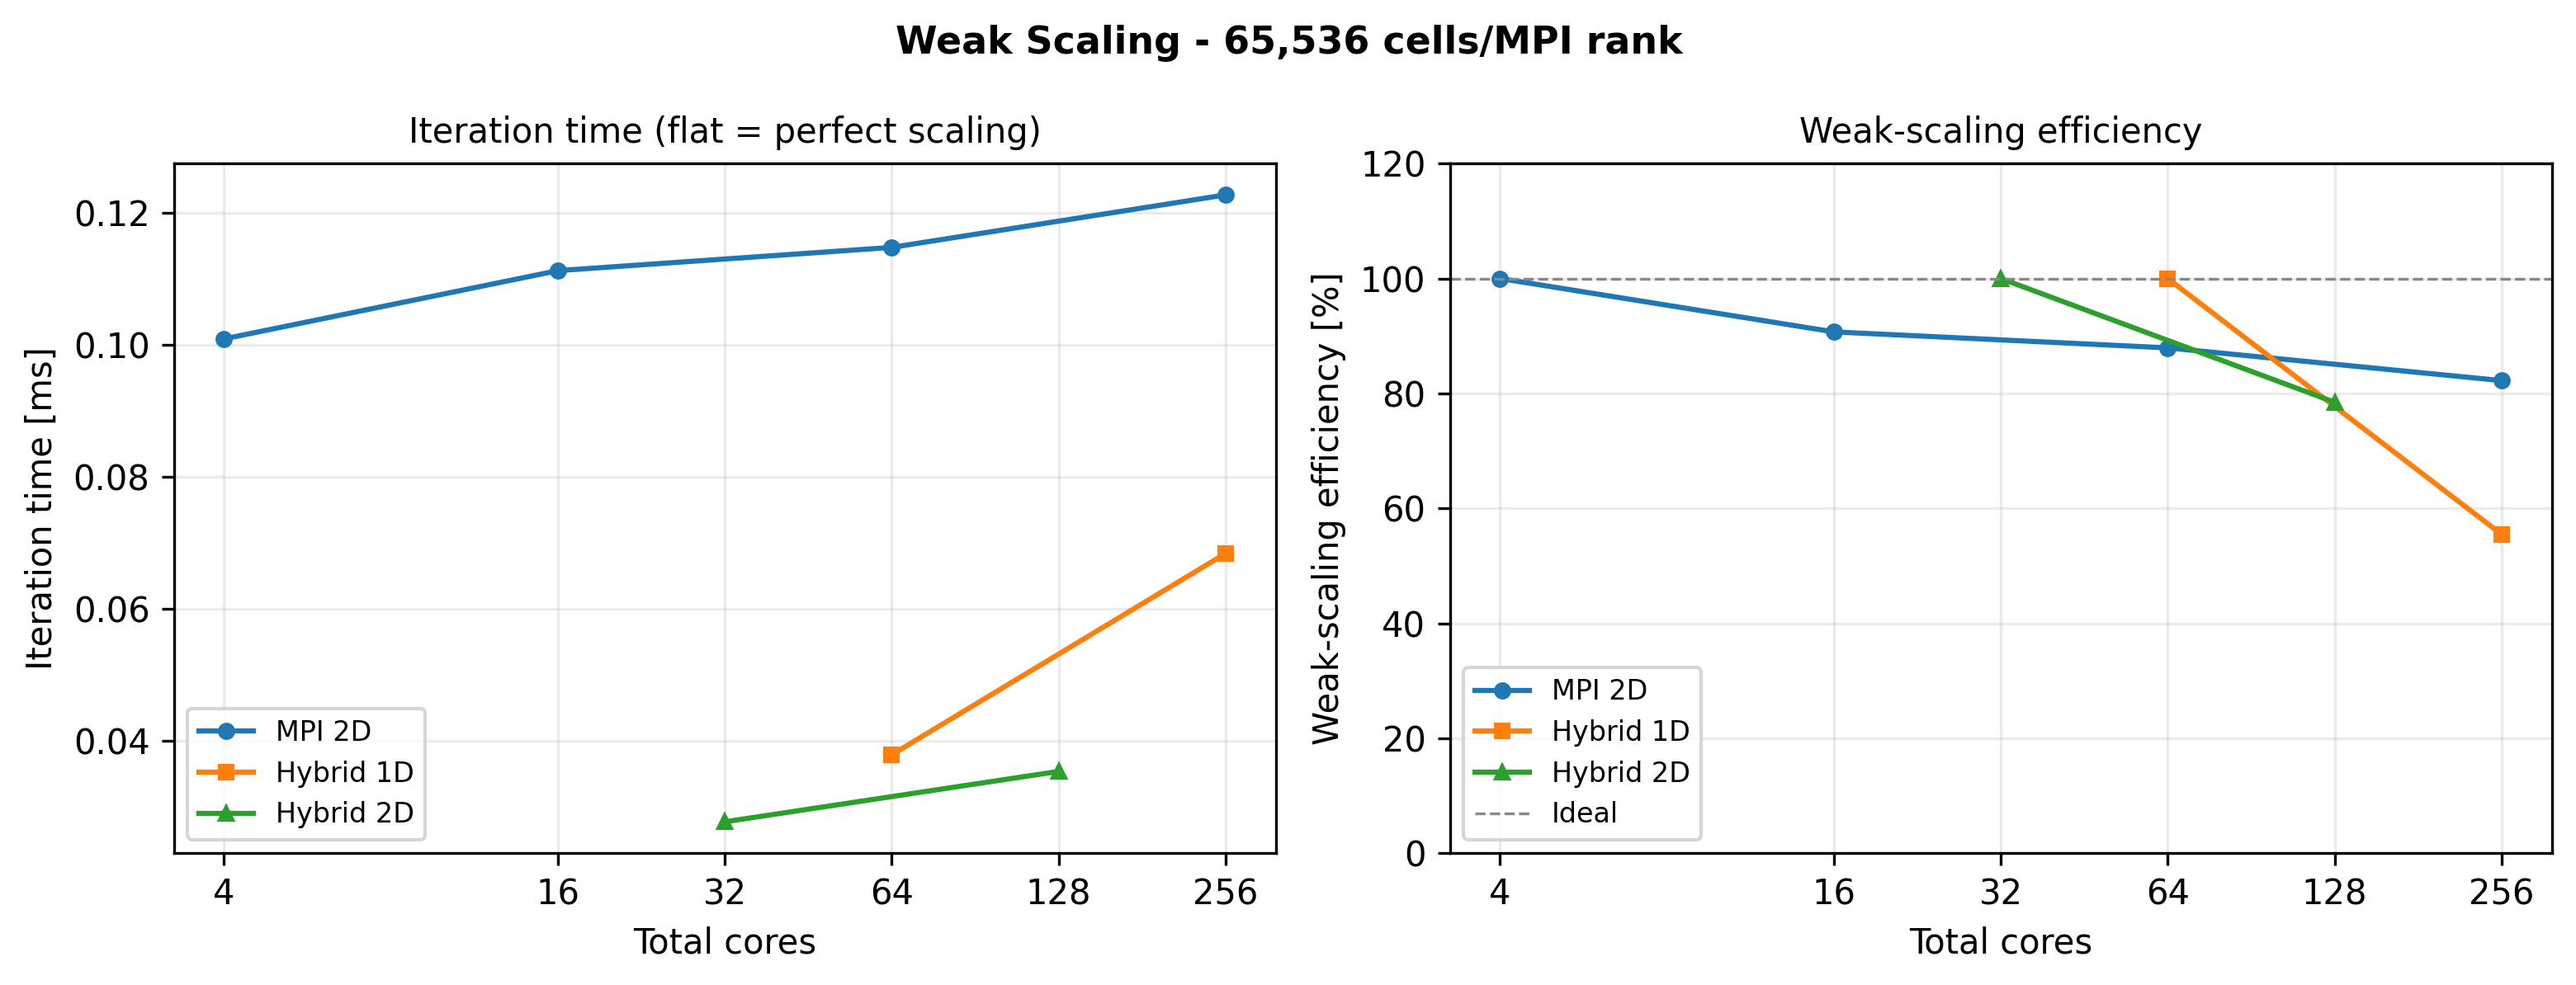
\includegraphics[width=0.8\textwidth]{docs/figures/ppp_weak_scaling.png}
    \caption{Slabé škálování (65\,536 buněk/rank): iterační čas (vlevo) mírně roste se
             zvyšováním $P$, efektivita (vpravo) klesá pod 100\,\% kvůli komunikační režii.
             2D dekompozice si drží lepší efektivitu než 1D.}
    \label{fig:weak_scaling}
\end{figure}

% =========================================================
\section{Profilování}
\label{sec:profilovani}
% =========================================================

\subsection{Vampir}
\label{subsec:vampir}

Trasování bylo provedeno pro konfiguraci P2P 2D, doména $1024^2$,
16 procesů, 100 iterací. Časová osa všech procesů
(obr.~\ref{fig:vampir_timeline}) ukazuje pravidelně se opakující
strukturu iterací, ve které se střídají fáze lokálního výpočtu
(hnědě) s fázemi MPI volání (modře). Hnědé bloky výpočtu zabírají
dominantní část plochy, modré bloky mají ale nezanedbatelnou délku,
především na konci každé iterace. Jde převážně o čekání
v \texttt{awaitHaloExchange} na synchronizaci se sousedy před další
iterací. Komunikační matice
(obr.~\ref{fig:vampir_commatrix}) zachycuje rozdíl mezi 1D a 2D
dekompozicí. V 1D vzniká úzký diagonální pás, neboť každý rank
komunikuje jen se dvěma sousedy v řadě, a maximum barevné škály
dosahuje 840\,KiB. 2D má širší vzor díky čtyřem sousedům dlaždice,
ale maximum škály klesá na 210\,KiB kvůli kratším hranám
($N/\sqrt{P}$ vs.\ $N$). Souhrn doby strávené v jednotlivých
funkcích na rank (obr.~\ref{fig:vampir_process_summary}) potvrzuje,
že \texttt{computePoint} dominuje napříč všemi 16 ranky s velmi
malými rozdíly mezi nimi.

\begin{figure}[H]
    \centering
    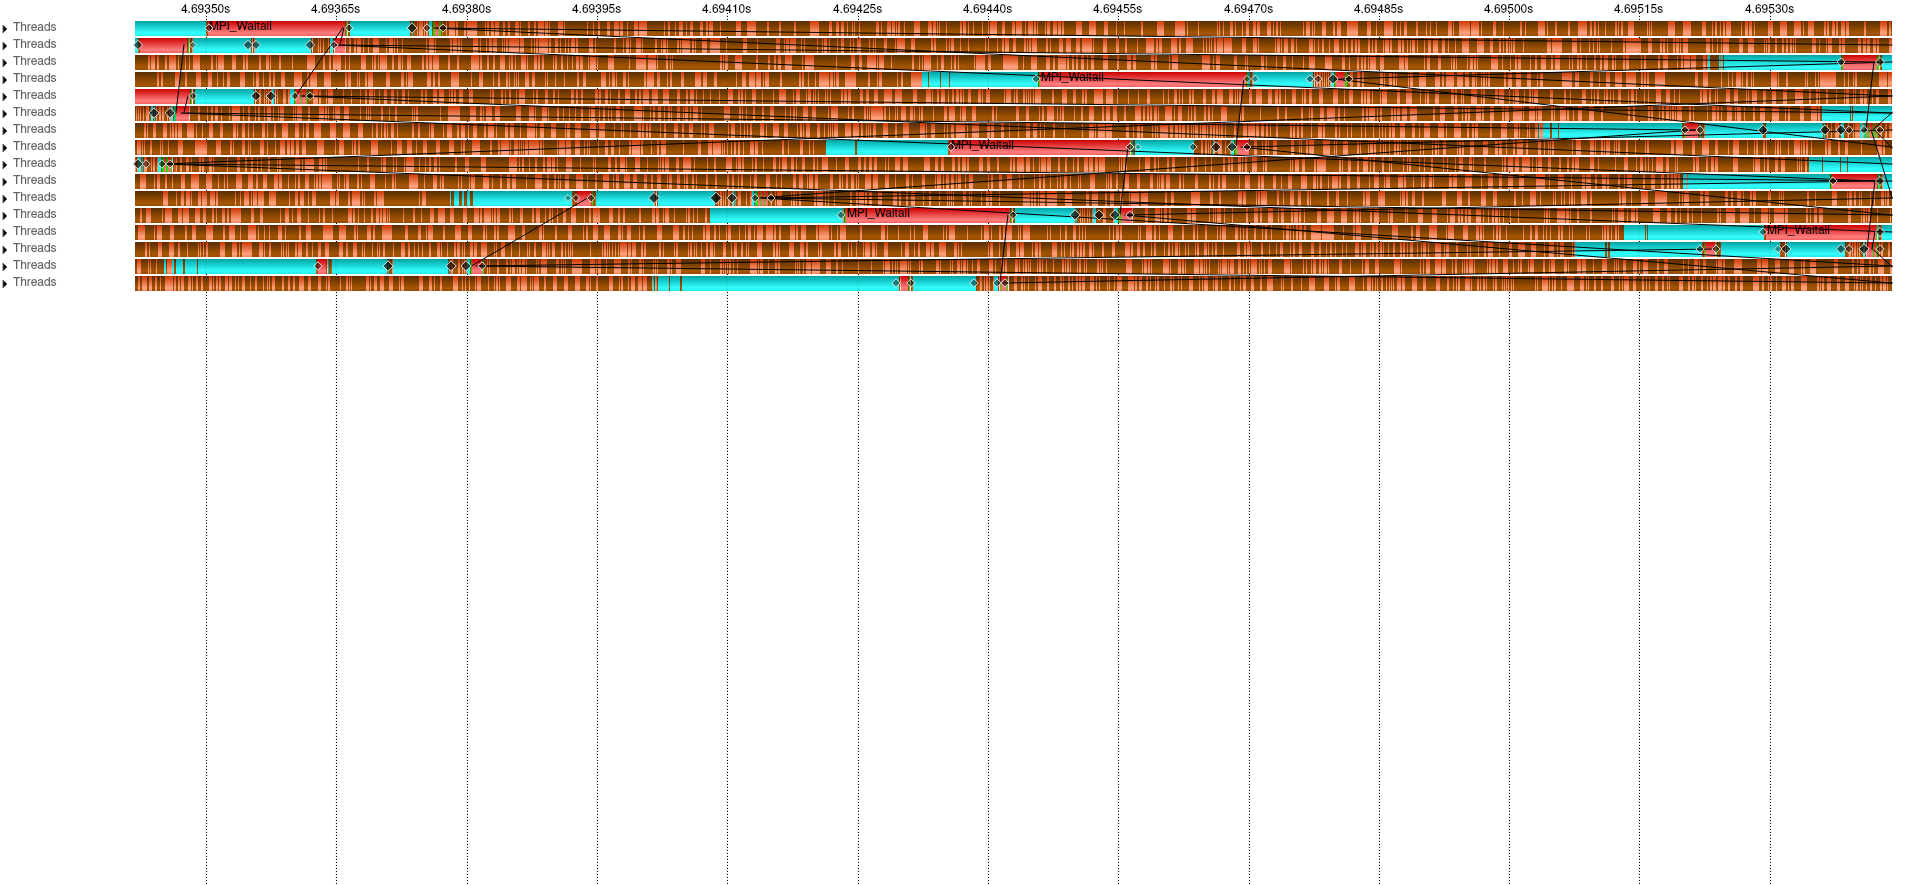
\includegraphics[width=0.9\textwidth]{docs/figures/scorep/Master_Timeline_p2p_2d_trace.png}
    \caption{Vampir Master Timeline (P2P, 2D, $1024^2$, 16 procesů, zoom na jednu iteraci).}
    \label{fig:vampir_timeline}
\end{figure}

\begin{figure}[H]
    \centering
    \begin{subfigure}{0.48\textwidth}
        \centering
        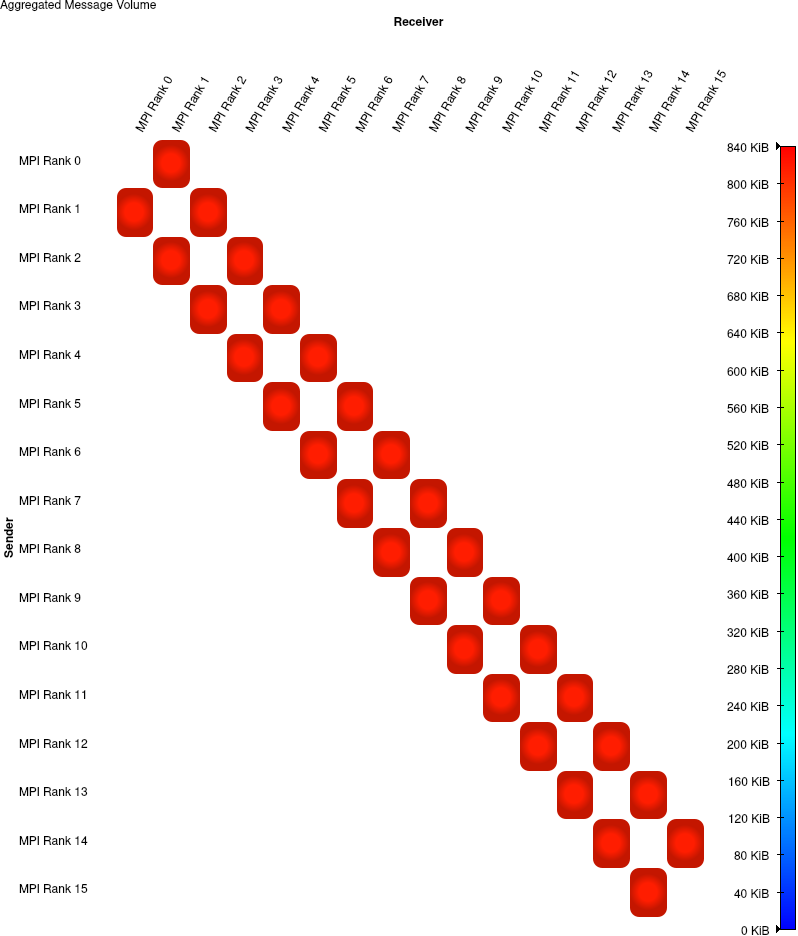
\includegraphics[width=\textwidth]{docs/figures/scorep/Communication_Matrix_View_p2p_1d_trace_2.png}
        \caption{1D dekompozice ($16\times1$).}
        \label{fig:commatrix_1d}
    \end{subfigure}
    \hfill
    \begin{subfigure}{0.48\textwidth}
        \centering
        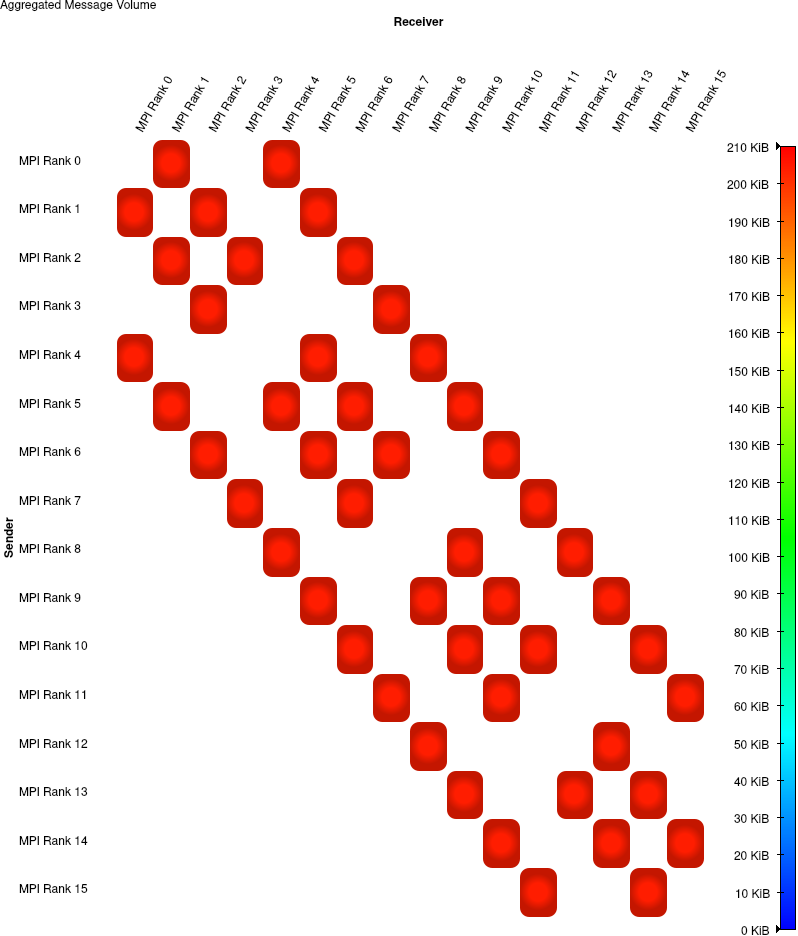
\includegraphics[width=\textwidth]{docs/figures/scorep/Communication_Matrix_View_p2p_2d_trace_2.png}
        \caption{2D dekompozice ($4\times4$).}
        \label{fig:commatrix_2d}
    \end{subfigure}
    \caption{Vampir Communication Matrix (Aggregated Message Volume), 16 procesů.}
    \label{fig:vampir_commatrix}
\end{figure}

\begin{figure}[H]
    \centering
    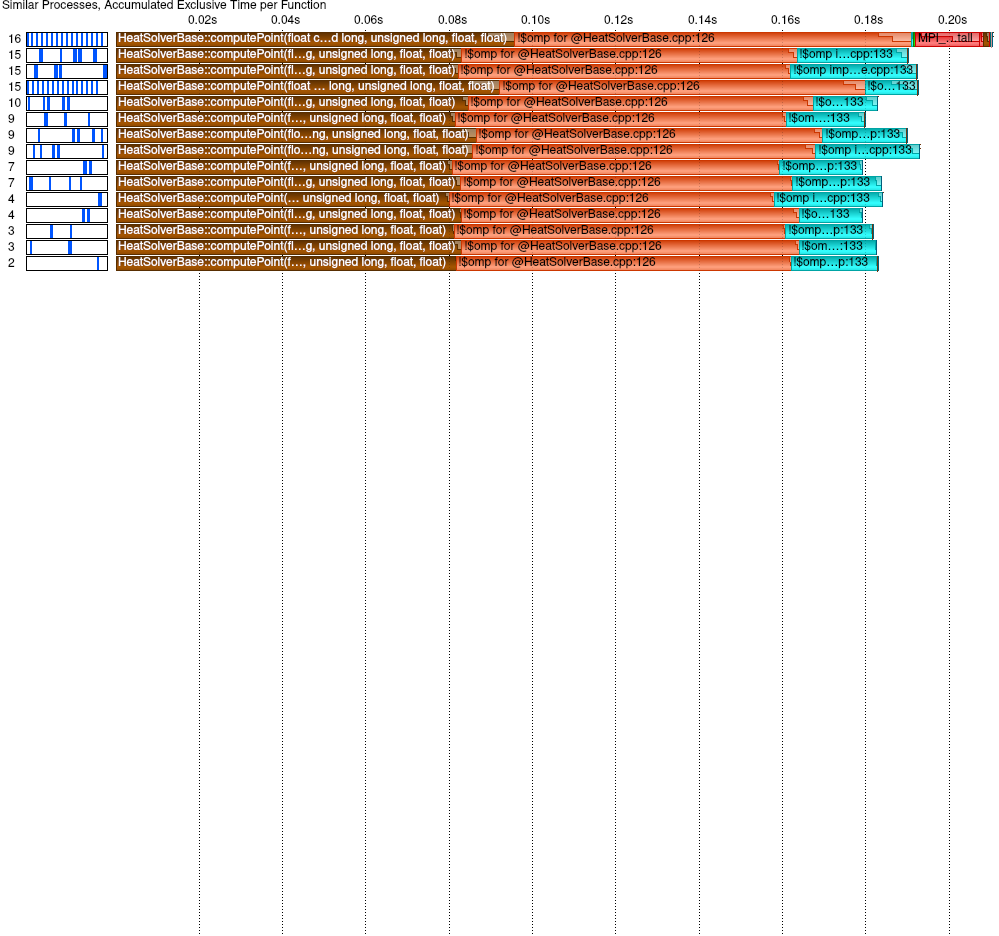
\includegraphics[width=0.85\textwidth]{docs/figures/scorep/Process_Summary_p2p_2d_trace.png}
    \caption{Vampir Process Summary, 16 procesů. Vyrovnaná zátěž, dominuje \texttt{computePoint}.}
    \label{fig:vampir_process_summary}
\end{figure}

\subsection{Cube}
\label{subsec:cube}

Pohled na kartézskou topologii procesů s metrikou \texttt{bytes\_sent}
ukazuje rovnoměrnost komunikace mezi procesy. Celkový objem zaslaných
MPI dat za celý běh je $2{,}68\times 10^7$\,B u 2D a
$4{,}18\times 10^7$\,B u 1D dekompozice, což odpovídá vyššímu
komunikačnímu objemu 1D (poměr halo částí
$V_\text{1D}/V_\text{2D} = \sqrt{P}/2 = 2$ pro $P=16$).
Topologie 2D (obr.~\ref{fig:cube_2d}) je zobrazena přes všechna
MPI volání, takže rank 0 vyniká kvůli scatter/gather a ostatních
15 ranků má téměř shodný objem halo komunikace. Topologie 1D
(obr.~\ref{fig:cube_1d}) je filtrovaná pouze na halo
\texttt{MPI\_Isend}, vnitřní ranky odesílají identický objem
(2 sousedi v řadě), krajní ranky 0 a 15 poloviční (1 soused).

\begin{figure}[H]
    \centering
    \begin{subfigure}{0.75\textwidth}
        \centering
        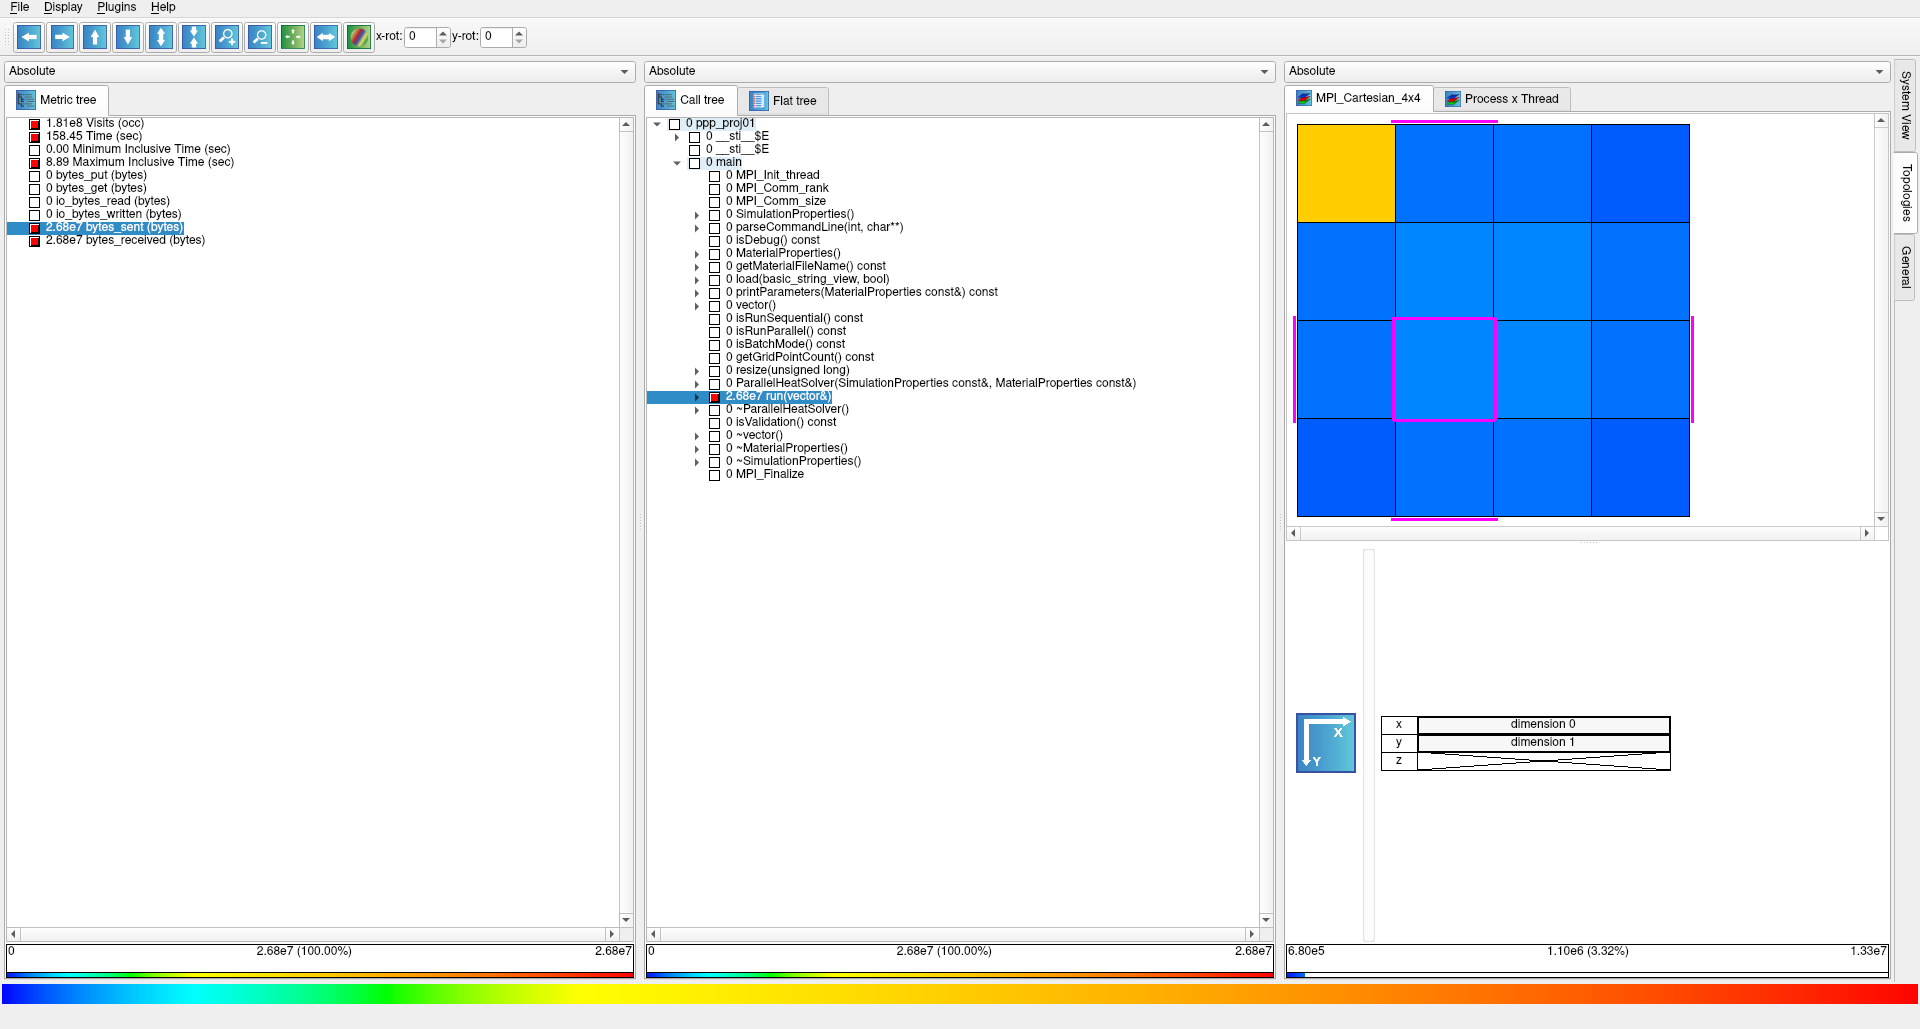
\includegraphics[width=\textwidth]{docs/figures/scorep/cube2.png}
        \caption{}
        \label{fig:cube_2d}
    \end{subfigure}
    \hfill
    \begin{subfigure}{0.75\textwidth}
        \centering
        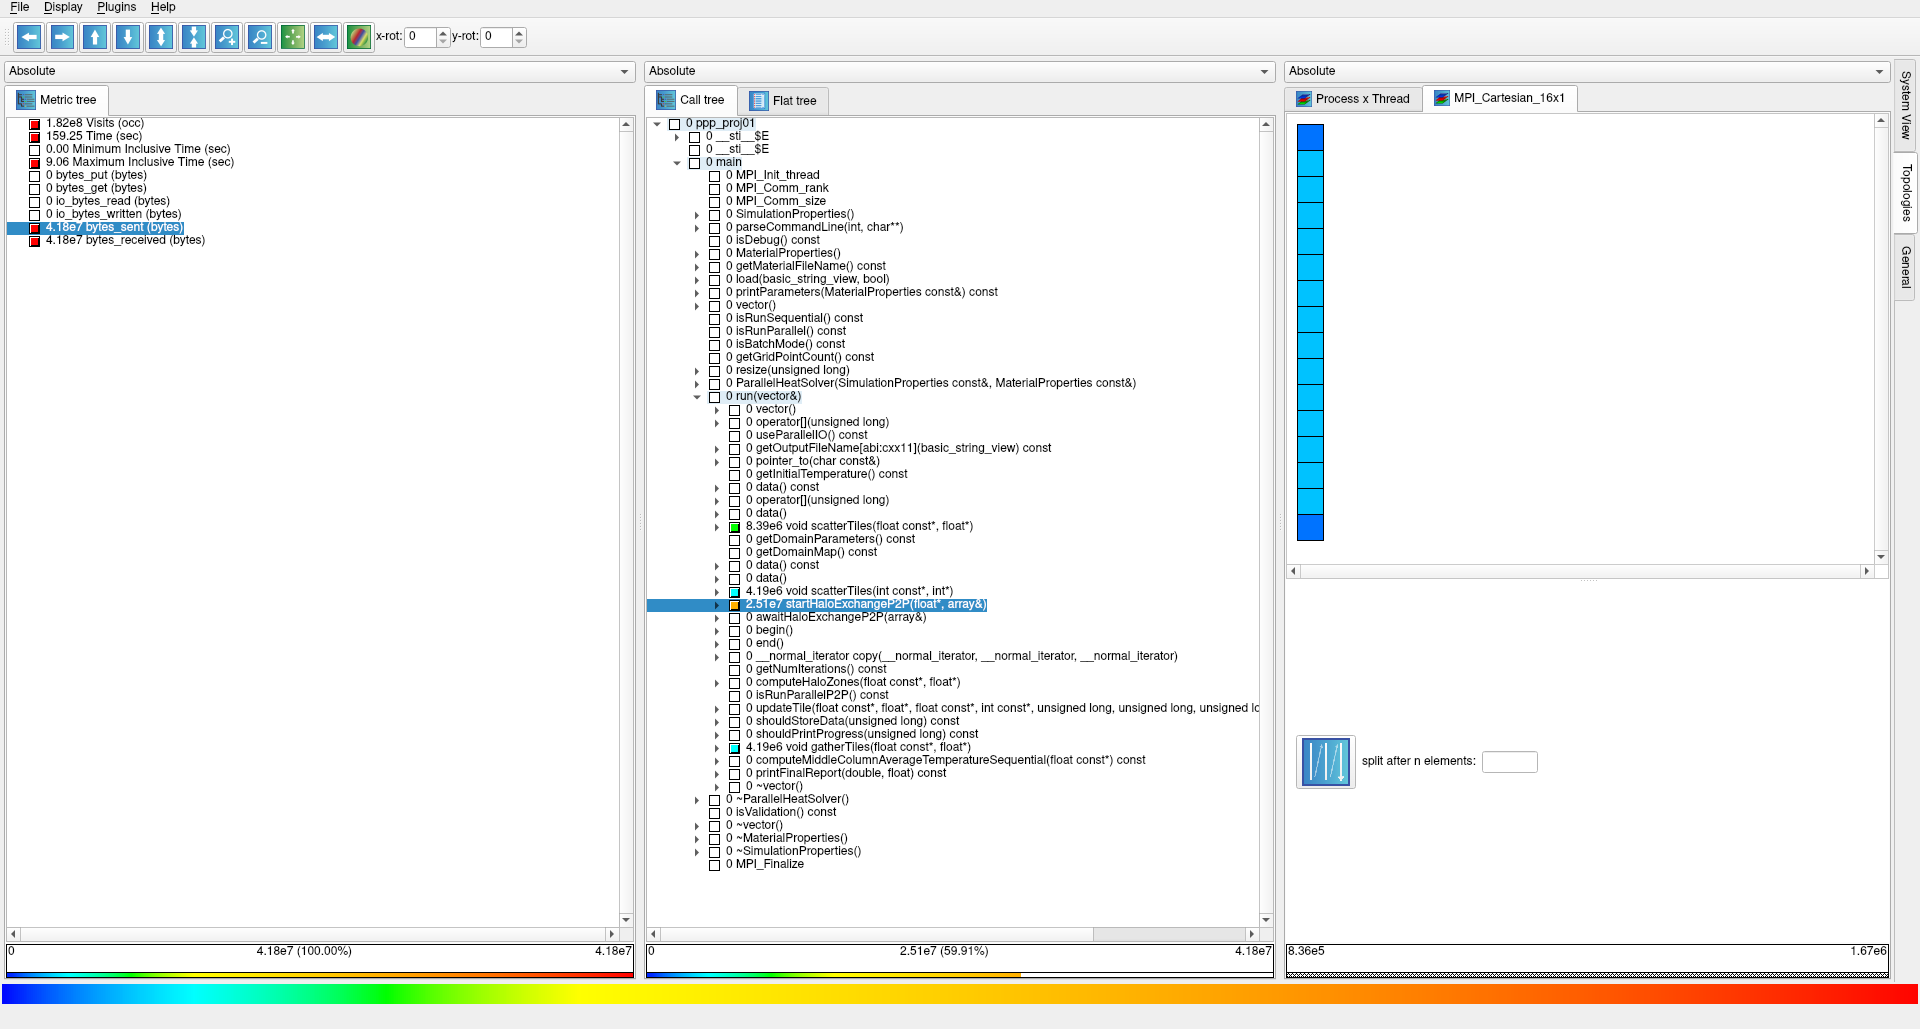
\includegraphics[width=\textwidth]{docs/figures/scorep/cube3.png}
        \caption{}
        \label{fig:cube_1d}
    \end{subfigure}
    \caption{Cube, kartézská topologie procesů s metrikou \texttt{bytes\_sent}, 16 procesů.}
    \label{fig:cube_topology}
\end{figure}

% =========================================================
\section{Závěr}
\label{sec:zaver}
% =========================================================

Implementace dosahuje superlineárního zrychlení $\sim 666\times$
(Hybrid 2D P2P, 256 jader, doména $4096^2$, bez I/O).
RMA výkon byl zlepšen celkově 133-268$\times$ oproti výchozímu stavu,
přičemž dominantním příspěvkem je nahrazení \texttt{MPI\_Get} za \texttt{MPI\_Put}
(55-80$\times$), sekundárně packing (1{,}5-3$\times$) a PSCW synchronizace
(1{,}15-1{,}74$\times$ dle počtu uzlů).
2D dekompozice překonává 1D v 63 z 90 přímých srovnání
díky $\sqrt{P}/2$-krát menšímu objemu komunikace na proces.
Oprava HDF5 chunkování a Lustre striping výrazně zrychlily paralelní zápis
oproti původní variantě s lokálními chunky. Pro měřené objemy dat ale
paralelní I/O stále zůstalo pomalejší než sekvenční zápis.

\end{document}
